%% 
%% Copyright 2024 by MDPI and authors. This is an open access article distributed under the 
%% Creative Commons Attribution License which permits unrestricted use, distribution, and 
%% reproduction in any medium, provided the original work is properly cited.
%%

\documentclass[computers,article,submit,pdftex,moreauthors]{Definitions/mdpi}

%% METADATA
\firstpage{1}
\pubvolume{1}
\issuenum{1}
\articlenumber{0}
\pubyear{2026}
\copyrightyear{2026}
\datereceived{} 
\daterevised{} 
\dateaccepted{} 
\datepublished{} 

%% The journal E-ISSN (2073-431X for Computers) is set automatically by the
%% "computers" class option above; no manual \ISSN command is required.

\usepackage[utf8]{inputenc}

%% TITLE AND AUTHOR INFORMATION
\Title{Occlusion-Robust Single-View 3D Reconstruction of Pigs via Discrete Latent Keypoint Completion and Skeleton Joint-Angle Constraints}

\Author{Ge Wang $^{1,2}$, Tao Zhu $^{1,2}$ and Fuchuan Ni $^{1,2,*}$}

\AuthorNames{Ge Wang, Tao Zhu and Fuchuan Ni}

\address{%
$^{1}$ \quad Key Laboratory of Intelligent Livestock Farming Technology, Ministry of Agriculture and Rural Affairs, Wuhan 430070, China\\
$^{2}$ \quad College of Informatics, Huazhong Agricultural University, Wuhan 430070, China}

\corres{Correspondence: fcni\_cn@mail.hzau.edu.cn (F.N.)}

%% ABSTRACT AND KEYWORDS
\abstract{Single-view 3D reconstruction of pigs provides structured information for posture analysis and precision livestock monitoring. However, images collected in real pig houses are rife with self-occlusion, inter-animal occlusion, and pen-rail occlusion, which often lead to missing 2D keypoints and unstable 3D pose regression, further causing implausible local rotations and anatomically inconsistent limb configurations. We propose an occlusion-robust single-view 3D reconstruction framework that couples a Discrete Latent Pose Completion Module (DLPCM) with a skeleton joint-angle constraint (SC). Unlike using DLPCM as a standalone 2D pose estimator, our framework only completes occluded keypoints with a codebook-driven masked fusion, while retaining the original SMAL-Pig predictions for visible keypoints. The SC applies weak priors on joint angles in the local pose parameter space of SMAL-Pig and does not impose bone-length or scale constraints. In the absence of dense 3D ground truth in real farm images, we evaluate from three complementary perspectives: 2D keypoint reprojection accuracy, silhouette consistency, and pose plausibility measured by the joint rotation violation rate (JRVR). Experiments on an occlusion-rich pig dataset show that DLPCM improves PCK from 61.85\% to 66.73\%, and IoU from 64.04\% to 67.90\%, while reducing JRVR from 69.74\% to 24.34\%. Adding SC further suppresses abnormal local rotations and achieves the lowest JRVR of 9.38\% with competitive PCK and IoU. These results indicate that DLPCM primarily enhances structural observations in occluded regions, whereas SC mainly improves pose plausibility; their combination yields a better balance between projection consistency and pose validity under occlusion.}

\keyword{pigs; single-view 3D reconstruction; occlusion-aware keypoint completion; skeleton joint-angle constraint; pose plausibility; weakly supervised animal reconstruction; silhouette consistency; JRVR}

\begin{document}

\section{Introduction}\label{sec:intro}

Precision livestock farming benefits from computer vision and deep learning for automatic monitoring of growth, behavior, and health status in swine production. Compared with 2D imagery, single-view 3D reconstruction provides richer geometric cues on body shape, limb connectivity, and spatial posture, enabling downstream analysis such as behavior recognition, morphometrics, and health assessment \cite{ref1,ref2,ref3,ref4,ref5,ref6,ref7,ref8,ref9,ref10}. However, real pig-house imagery often contains self-occlusion, inter-animal occlusion, and pen-rail occlusion. These factors cause missing 2D keypoints and unstable 3D pose regression, which manifest as implausible local rotations and anatomically inconsistent limb configurations.

Existing animal 3D reconstruction approaches fall into three families: depth/point-cloud reconstruction, multi-view geometric reconstruction, and single-view reconstruction. Depth sensing with RGB-D or ToF sensors can directly capture geometry and enable point-cloud processing (registration, filtering, segmentation, surface reconstruction) \cite{ref11,ref12,ref13,ref14}. Yet, in dusty, humid, and crowded barns with rails, point clouds are often incomplete or noisy, degrading stability. Multi-view methods leverage synchronized cameras, calibration, cross-view matching, and triangulation for 3D keypoints or skeletons \cite{ref15,ref16,ref17,ref18}, and can deliver accurate animal kinematics \cite{ref6}. However, these systems require careful camera setups and maintenance, raising deployment costs and limiting scalability in large-scale farms.

Single-view approaches are attractive due to their low hardware cost and easy integration with existing surveillance infrastructures. Parameterized models have catalyzed progress in this direction. SMPL captures articulated human shape and pose in a compact parameterization \cite{ref19}, while SMAL extends parameterized modeling to quadrupeds \cite{ref20,ref21,ref22,ref23,ref24}. Building on these foundations, researchers have developed animal-specific pipelines and priors to stabilize reconstruction without dense 3D supervision \cite{ref25,ref26}. Nevertheless, for pigs---an economically important species---robust single-view reconstruction under occlusion remains underexplored.

We address this gap by proposing an occlusion-robust single-view reconstruction framework for pigs that integrates a Discrete Latent Pose Completion Module (DLPCM) with a skeleton joint-angle constraint (SC). DLPCM follows a masked fusion design: visible keypoints predicted by the SMAL-Pig keypoint head are preserved, while occluded keypoints are completed via a vector-quantized latent codebook informed by predicted visibility masks \cite{ref28}. SC imposes weak priors on local joint angles in the SMAL-Pig pose parameter space, explicitly avoiding bone-length or scale constraints so that inter-individual shape variation is preserved.

In the absence of dense 3D ground truth for farm images, we evaluate from three complementary perspectives: (i) 2D keypoint reprojection accuracy (PCK), (ii) silhouette consistency (IoU), and (iii) pose plausibility via the Joint Rotation Violation Rate (JRVR). On an occlusion-rich pig dataset, DLPCM improves PCK from 61.85\% to 66.73\% and IoU from 64.04\% to 67.90\%, while reducing JRVR from 69.74\% to 24.34\%. Adding SC further suppresses abnormal local rotations and achieves the lowest JRVR of 9.38\% with competitive PCK and IoU.

The main contributions are as follows:

\begin{enumerate}
  \item An occlusion-robust single-view 3D reconstruction framework for pigs that enhances the completeness of 2D structural observations under occlusion.
  \item A masked-fusion integration of DLPCM into the SMAL-Pig pipeline that preserves visible keypoints while completing only occluded ones using a vector-quantized latent codebook.
  \item A skeleton joint-angle constraint that regularizes local rotations to curb anatomically implausible configurations without enforcing bone-length or scale constraints.
  \item Comprehensive evaluation with keypoint accuracy, silhouette consistency, and pose-plausibility metrics, including ablations and sensitivity analyses.
\end{enumerate}

\section{Materials and Methods}\label{sec:materials}

\subsection{Dataset and Annotations}\label{sec:dataset}

The dataset comprises 2,708 pig images collected at the Huazhong Agricultural University experimental pig farm (Wuhan, China), covering common breeds such as Erhualian and Hubei White. Hikvision smart cameras were installed in the measuring room, farrowing room, sow room, and replacement room. Images were extracted as keyframes from surveillance videos recorded between September 2021 and June 2023 at a resolution of 2560 $\times$ 1440 pixels; cameras were mounted overhead or obliquely to capture diverse postures.

In total, 7,672 pig instances were annotated across the 2,708 images using Labelme, including 1,524 daytime and 1,184 nighttime images. Each image includes keypoint and silhouette annotations. Examples are shown in Figure~\ref{fig:dataset}.

\begin{figure}[H]
\centering
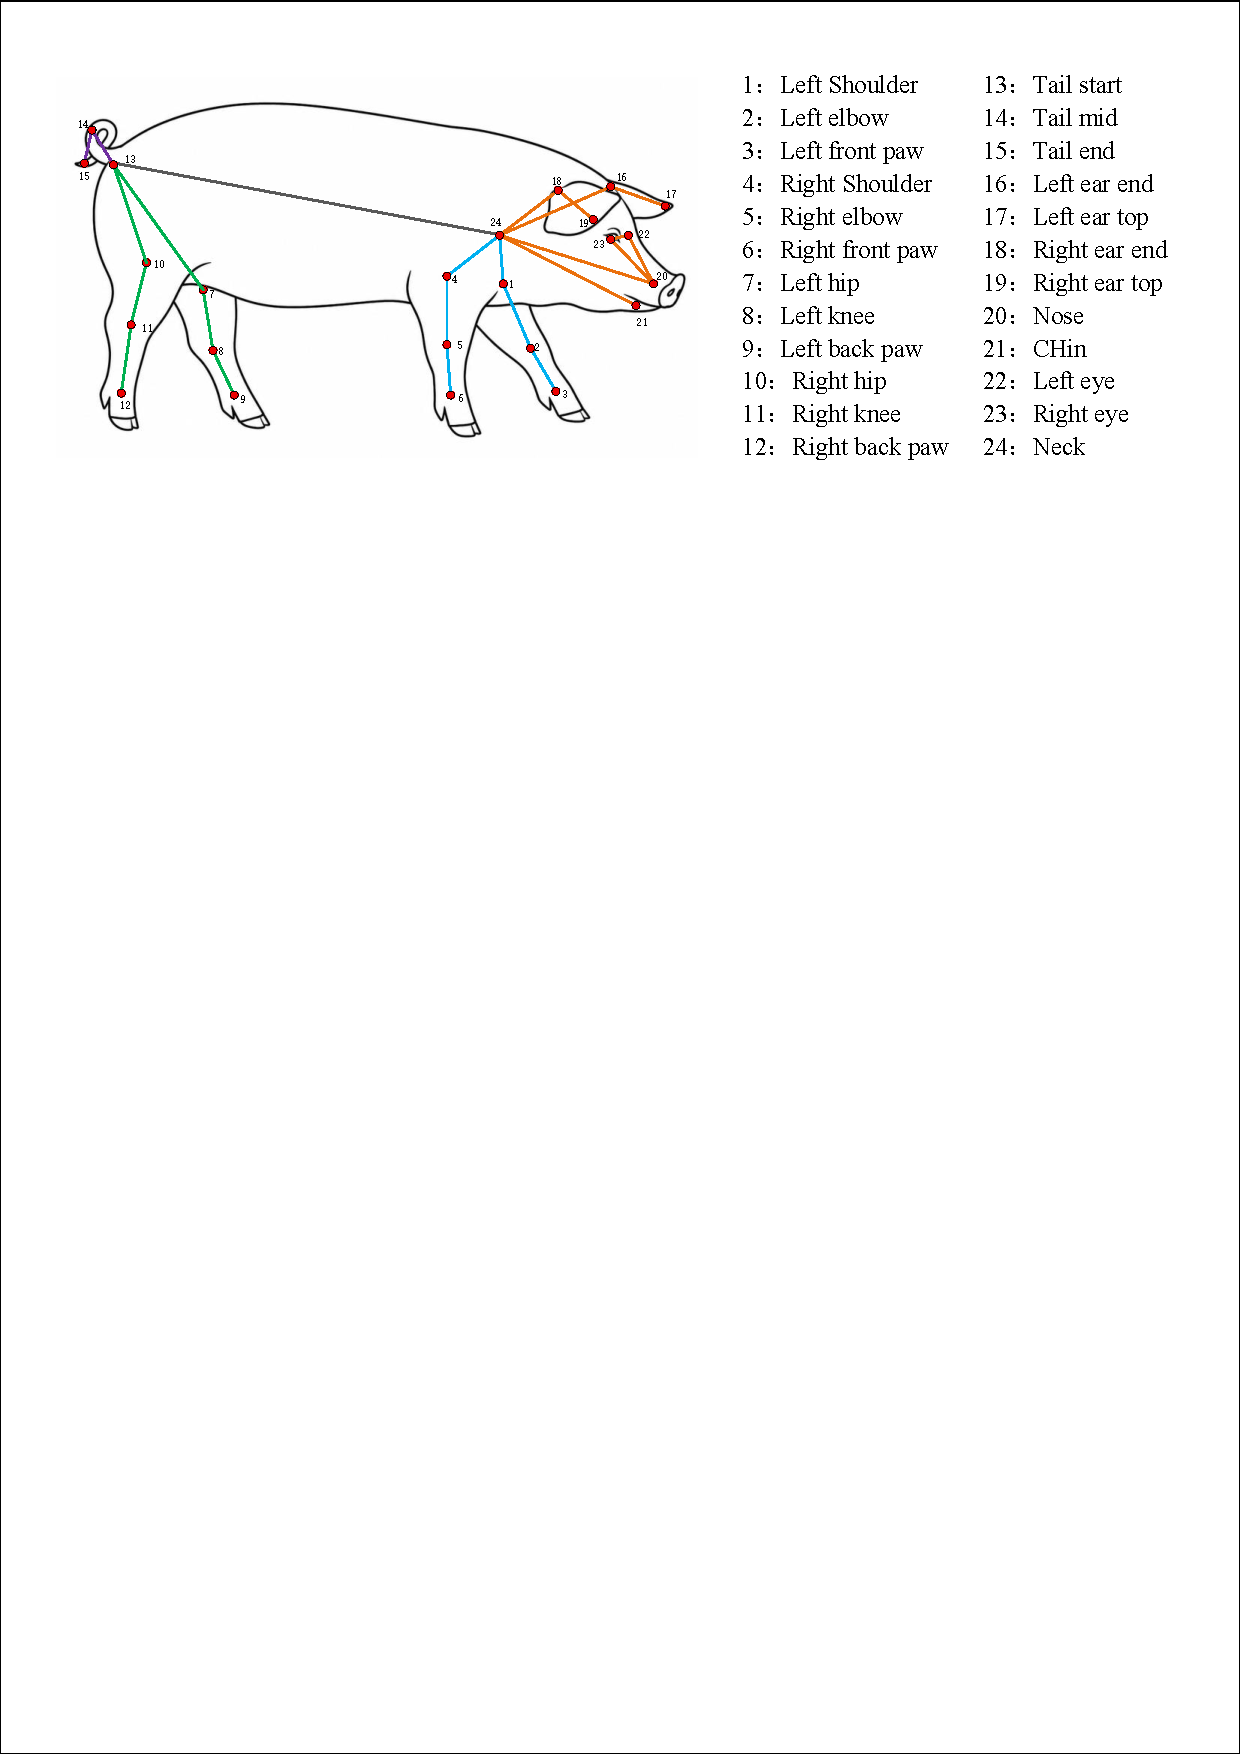
\includegraphics[width=\textwidth,trim=1cm 21cm 1cm 1cm,clip]{fig/KeyPoint.pdf}
\caption{Examples of annotated pig images covering diverse poses and occlusion types, including self-occlusion, inter-animal occlusion, and pen-rail occlusion. Images were collected from real pig-house environments under varying illumination.}
\label{fig:dataset}
\end{figure}

We randomly split the dataset into training/validation/test sets with a 6:3:1 ratio, resulting in 1,625/812/271 images, respectively. Data augmentation included Gaussian noise and random channel brightness adjustments to improve robustness to weak signals and illumination variations in barns.

To enrich occlusion patterns, we retained natural occlusions and synthesized pseudo occlusions by overlaying opaque black square blocks of 30 pixels per side on a grid. Adjacent blocks are spaced by 200 pixels horizontally and vertically, yielding a 230-pixel grid step. Blocks start from the top-left corner and are clipped at image boundaries. According to manual visibility labels, occluded keypoints account for 21.1\% of all annotated keypoints, whereas visible keypoints account for 78.9\%, increasing the difficulty of pose estimation and 3D reconstruction. Synthetic blocks were not used as oracle visibility indicators during testing.

Manual visibility labels were used only to supervise the GK-HourGlass visibility branch during training. In validation and testing, DLPCM builds masks from visibility vectors predicted by GK-HourGlass rather than using manual visibility labels directly. Consequently, the evaluation corresponds to an automatic-inference setting rather than an oracle setting.

\subsection{Single-View 3D Reconstruction Network for Pigs}\label{sec:smal_pig}

\begin{figure}[H]
\centering
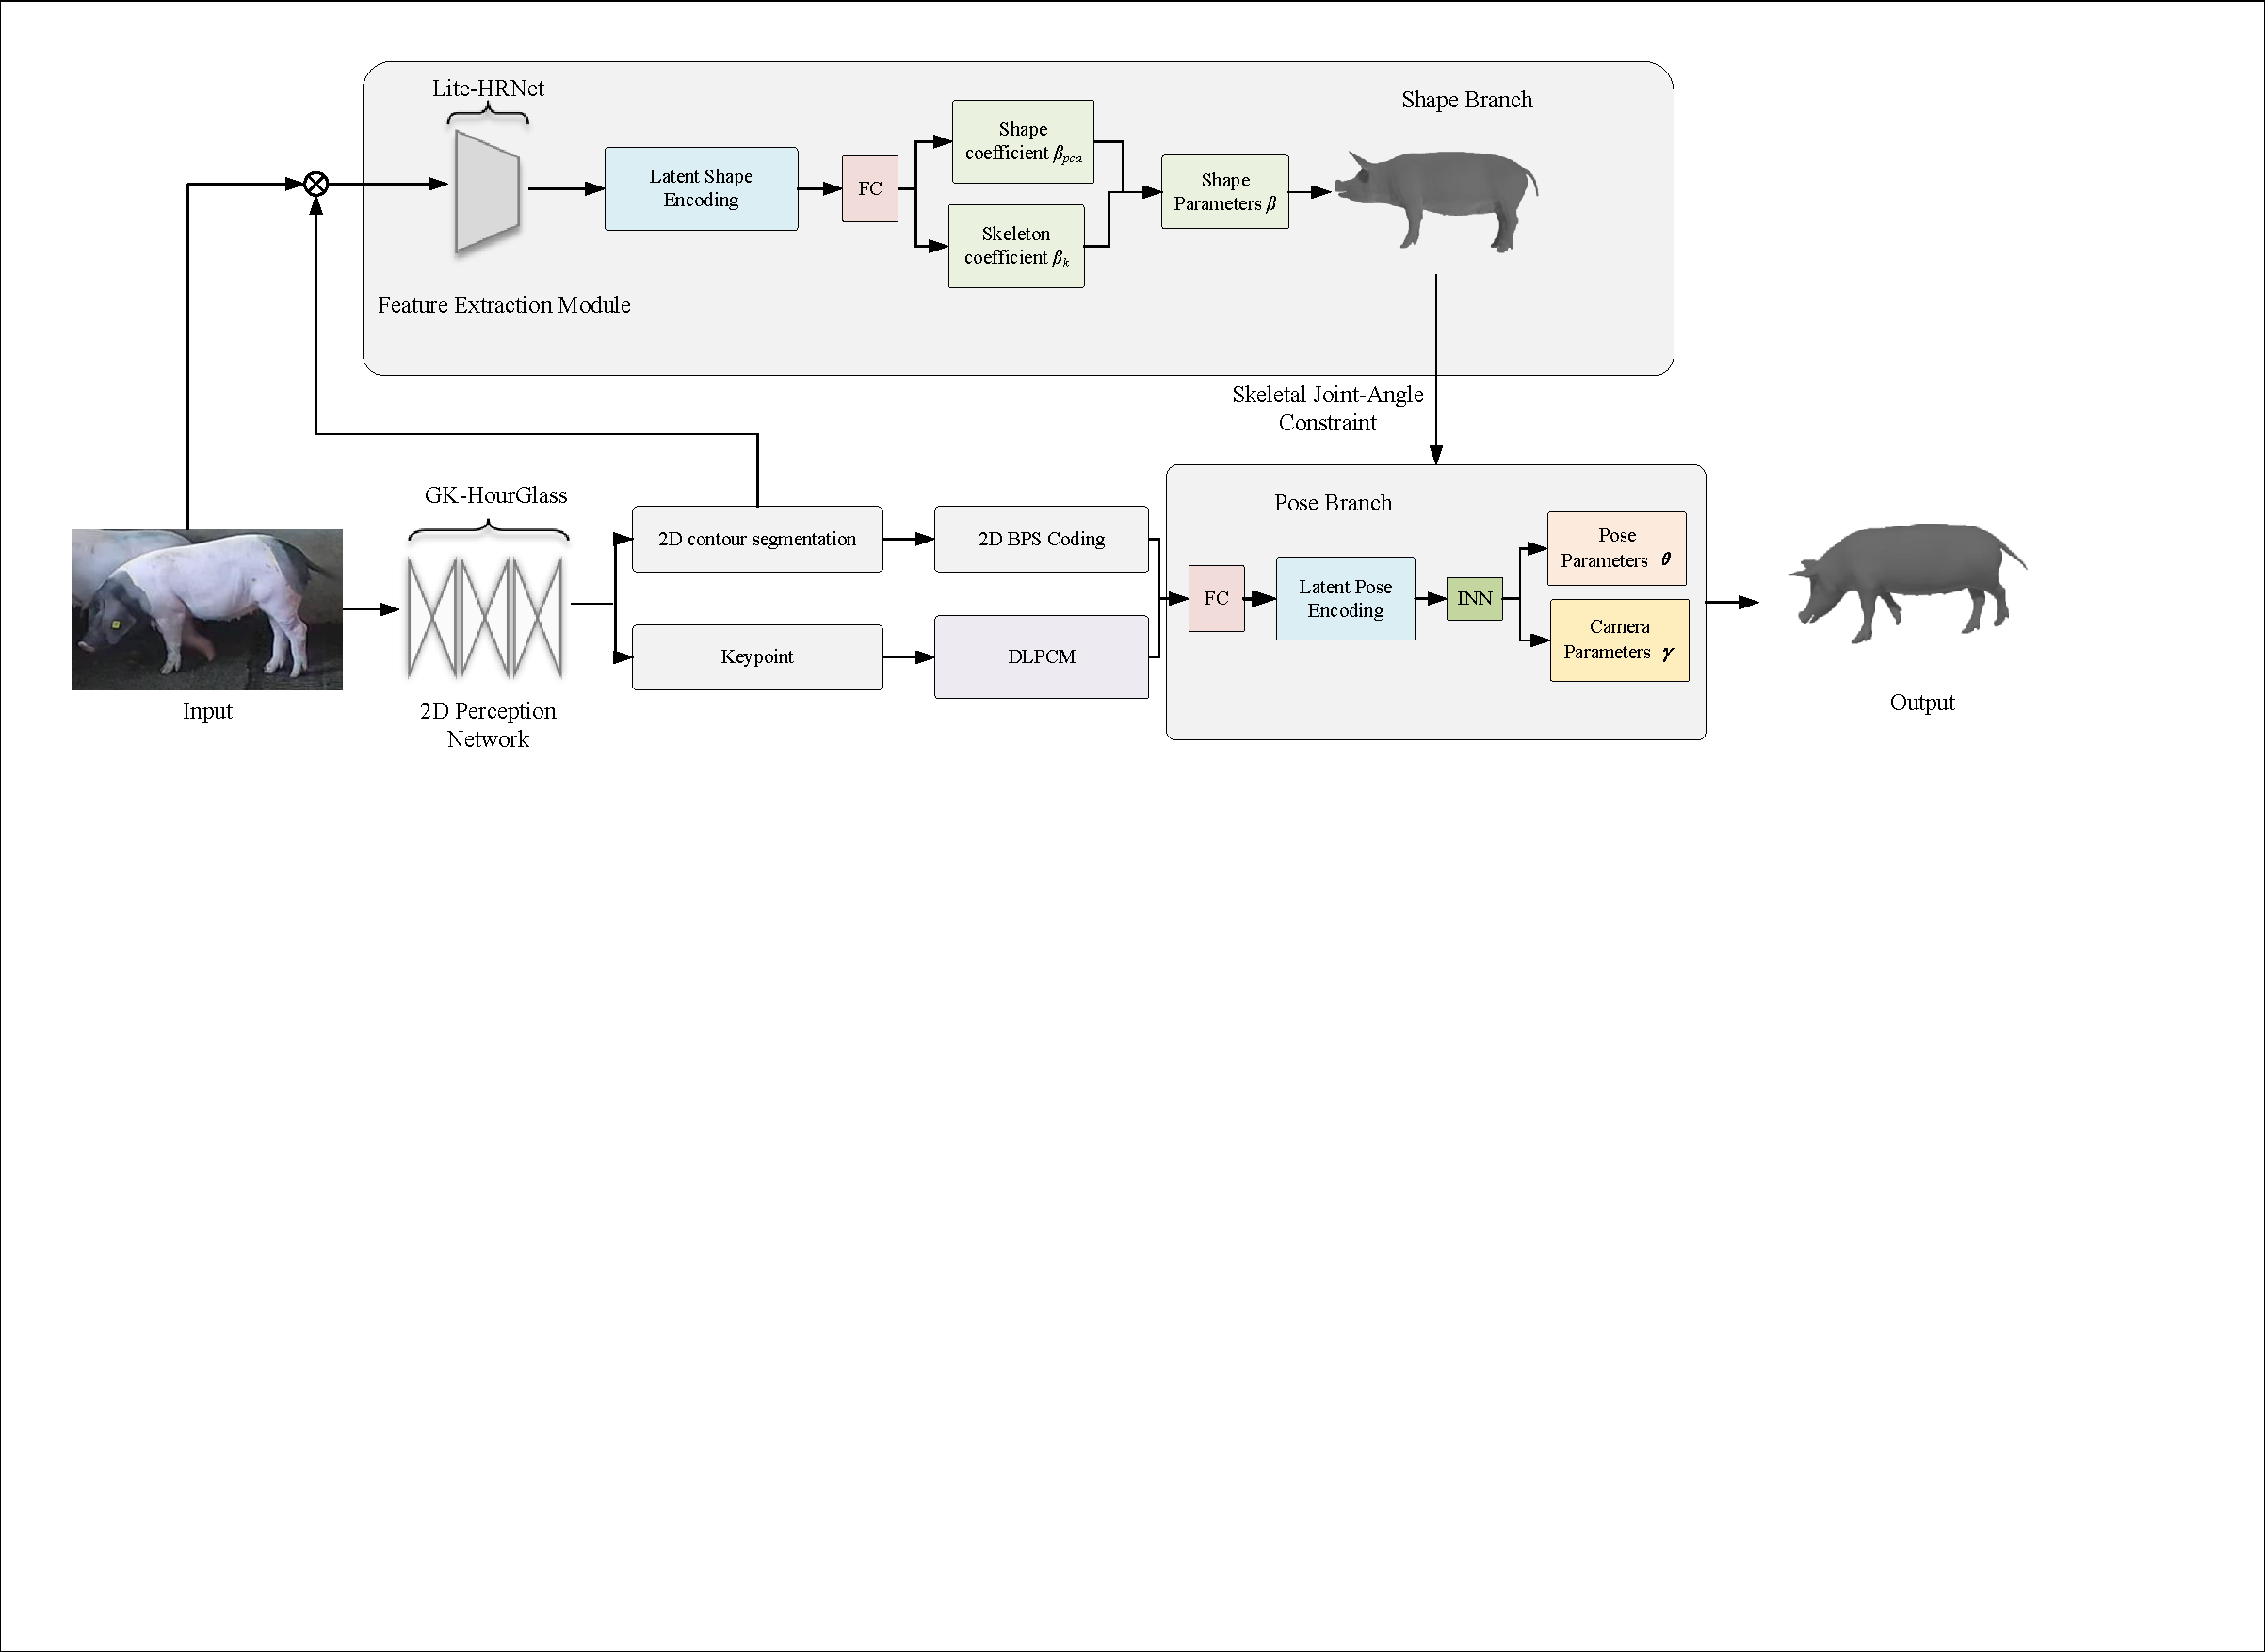
\includegraphics[width=\textwidth,trim=1cm 16cm 1cm 1cm,clip]{fig/fig2.pdf}
\caption{Occlusion-robust single-view 3D reconstruction network for pigs. FC denotes a fully connected layer and INN denotes an invertible neural network. A 2D feature extractor (GK-HourGlass) predicts keypoints and silhouettes; conditioned on these observations, dedicated heads regress shape, pose, and camera parameters before SMAL-Pig synthesizes the final mesh. DLPCM completes occluded keypoints and SC regularizes local joint rotations.}
\label{fig:smal_pig_network}
\end{figure}

To enable single-view 3D reconstruction of pigs, we follow a BARC-style weakly supervised pipeline and adapt a SMAL-based parametric model to porcine morphology (SMAL-Pig). SMAL-Pig aligns the SMAL articulated topology with a pig-specific template mesh and skeleton, preserves linear blend skinning, and represents inter-individual shape and local joint rotations with low-dimensional parameters. This formulation turns reconstruction into regressing shape, pose, and camera parameters rather than predicting dense geometry, yielding compact, anatomically consistent, and interpretable structure for quadrupeds with stable skeletal topology.

In the baseline network, the input is a single RGB image of a pig, and the outputs are shape, pose, and camera parameters. Following BARC, training relies primarily on 2D supervision without dense 3D ground truth: a 2D feature extractor encodes multi-scale visual cues and predicts structural observations (keypoints and silhouettes). Conditioned on these observations, dedicated heads regress shape, pose, and camera parameters---using invertible neural networks (INNs) in the parameterization---before SMAL-Pig synthesizes the final mesh. The overall pipeline is illustrated in Figure~\ref{fig:smal_pig_network}.

\subsection{Occlusion-Robust Reconstruction Framework}\label{sec:occlusion_framework}

Occlusion is the principal cause of implausible reconstructions in single-view settings because it compromises the completeness of 2D observations. For nonrigid targets like pigs, directly regressing 3D pose from only visible regions makes the model susceptible to local texture noise, missing keypoints, and insufficient context, often yielding reverse bending, over-rotation, or local twisting.

To improve stability and pose plausibility under occlusion, we augment the baseline with a Discrete Latent Pose Completion Module (DLPCM) and a skeleton joint-angle constraint (SC). DLPCM completes occluded keypoints at the 2D observation level to strengthen the constraints for 3D regression, while SC regularizes local joint rotations in the pose parameter space to suppress reverse bending, excessive rotation, and local twisting. The two modules address complementary aspects---projection consistency and pose plausibility---and thus should be interpreted jointly rather than in isolation.

\subsection{Discrete Latent Pose Completion Module (DLPCM)}\label{sec:dlpcm}

DLPCM is not a standalone 2D pose estimator but a masked keypoint fusion mechanism. Inspired by neural discrete representation learning for occluded pig pose estimation \cite{ref28}, it is integrated into the SMAL-Pig pipeline. Classic codebook-based strategies can infer missing keypoints from visible structure, but using a limited codebook to predict all keypoints may bias even reliably detected visible keypoints when coverage is insufficient. Therefore, DLPCM preserves SMAL-Pig keypoint-head predictions for visible keypoints and completes only occluded ones with the discrete latent codebook. We employ GK-HourGlass as the improved HourGlass backbone to extract image features and jointly predict 2D keypoints and their visibilities. The initial keypoint set is defined as:

\begin{equation}
K_{\text{init}} = \{(x_1, y_1), (x_2, y_2), \ldots, (x_N, y_N)\}
\end{equation}

where $N$ denotes the number of keypoints for a pig, set to $N = 24$ in this work. $K_{\text{init}}$ represents the initial keypoint set, and $(x_i, y_i)$ denotes the coordinates of the $i$-th keypoint in the image plane. For neural network processing, we vectorize the keypoint coordinates as:

\begin{equation}
K_{\text{init}} = [x_1, y_1, x_2, y_2, \ldots, x_N, y_N]
\end{equation}

To distinguish between reliably observed and occluded keypoints, we introduce a visibility vector automatically predicted by GK-HourGlass:

\begin{equation}
V = [v_1, v_2, \ldots, v_N]
\end{equation}

where $v_i$ denotes the predicted visibility of the $i$-th keypoint. When GK-HourGlass predicts the keypoint as visible in the image, $v_i = 1$; otherwise, $v_i = 0$. During training, manual visibility labels supervise the visibility prediction branch. During validation and testing, we use only the network-predicted visibility vectors without relying on manual annotations.

Since each keypoint has two coordinate components ($x$ and $y$), we expand the visibility vector to a coordinate-level mask $M_v$ as:

\begin{equation}
M_v = [v_1, v_1, v_2, v_2, \ldots, v_N, v_N]
\end{equation}

The input to DLPCM consists of the initial keypoint coordinates and the predicted visibility mask:

\begin{equation}
X = [K_{\text{init}}, M_v]
\end{equation}

By combining keypoint coordinates and predicted visibility masks, we treat keypoints predicted as visible by GK-HourGlass as reliable observations, while sending occluded or invisible keypoints to DLPCM for completion. This strategy avoids treating occluded regions as reliable observations. Since the inference-time masks come from the keypoint detection network rather than manual annotations, DLPCM does not rely on oracle occlusion information. The mask provides only 2D visibility cues without 3D pose ground truth. Thus, DLPCM should be understood as inferring missing 2D observations from visible keypoint structure, not as providing direct 3D supervision.

During pose completion, we first pass the input keypoint information $X$ to an encoder to obtain a continuous latent representation:

\begin{equation}
z_e = E(X)
\end{equation}

where $E(\cdot)$ denotes the encoder function, and $z_e$ is the continuous latent vector output by the encoder, which captures global pose structure inferred from visible keypoints. To learn discrete pose patterns, we introduce vector quantization to map the continuous latent vector to the nearest neighbor in a predefined pose codebook:

\begin{equation}
C = \{e_1, e_2, \ldots, e_K\}, \quad e_j \in \mathbb{R}^d
\end{equation}

The codebook contains $K$ codebook vectors of dimension $d$, each corresponding to a typical pig pose pattern. We quantize the encoder output via nearest-neighbor lookup:

\begin{equation}
z_q = e_k, \quad k = \arg\min_j \|z_e - e_j\|_2
\end{equation}

where $k$ is the index of the nearest codebook vector to $z_e$, and $z_q$ is the quantized discrete latent pose representation. This operation maps continuous pose features to discrete pose structure space, helping the model learn stable structural relations among keypoints and improving the robustness of occluded keypoint completion.

The decoder then predicts complete keypoint coordinates from the quantized latent vector:

\begin{equation}
K_{\text{comp}} = D(z_q)
\end{equation}

where $D(\cdot)$ denotes the decoder function and $K_{\text{comp}}$ is the set of complete keypoints inferred from the discrete latent pose vector. To prevent visible keypoints from being replaced by completion results, we perform mask-based fusion to obtain the final keypoint set:

\begin{equation}
K_{\text{final}} = M_v \odot K_{\text{init}} + (1 - M_v) \odot K_{\text{comp}}
\end{equation}

Here, $K_{\text{final}}$ is the final keypoint set, $M_v$ is the coordinate-level visibility mask, and $\odot$ denotes element-wise multiplication. $K_{\text{init}}$ comes from the SMAL-Pig keypoint detection head, while $K_{\text{comp}}$ is reconstructed by the discrete latent pose completion network. This mask-based fusion strategy does not directly replace all keypoints with $K_{\text{comp}}$; instead, it retains $K_{\text{init}}$ for visible keypoints and uses $K_{\text{comp}}$ only for occluded keypoints. This design avoids reconstruction bias on visible keypoints due to limited codebook capacity, while preserving the ability of discrete latent pose learning to infer missing structure under occlusion.

The keypoint completion loss for DLPCM is defined as:

\begin{equation}
L_{\text{comp}} = \left[\frac{1}{\sum_i^N (1 - v_i)}\right] \sum_i^N (1 - v_i) \|K_{\text{comp},i} - K_{\text{gt},i}\|_2^2
\end{equation}

where $K_{\text{gt},i}$ denotes the ground-truth location of the $i$-th keypoint. This loss primarily acts on occluded keypoints, guiding the model to infer invisible keypoint positions from visible keypoints and global pig pose structure. If training samples contain no occluded keypoints, we use mean squared error over all keypoints as the completion supervision to avoid division by zero.

For the vector quantization process, we further introduce codebook loss and commitment loss:

\begin{equation}
L_{\text{vq}} = \|\text{sg}[z_e] - z_q\|_2^2 + \beta_{\text{vq}} \|z_e - \text{sg}[z_q]\|_2^2
\end{equation}

where $\text{sg}[\cdot]$ denotes the stop-gradient operation and $\beta_{\text{vq}}$ is the commitment loss weight. The first term updates the codebook vectors, while the second term constrains the encoder output to stay close to the corresponding codebook vector, improving the stability of discrete pose representation.

The total training loss for DLPCM is:

\begin{equation}
L_{\text{DLPCM}} = L_{\text{comp}} + \lambda_{\text{vq}} L_{\text{vq}}
\end{equation}

After training, DLPCM generates the fused keypoint set $K_{\text{final}}$, which is then used as structural observations for the subsequent 3D reconstruction stage.

\begin{figure}[H]
\centering
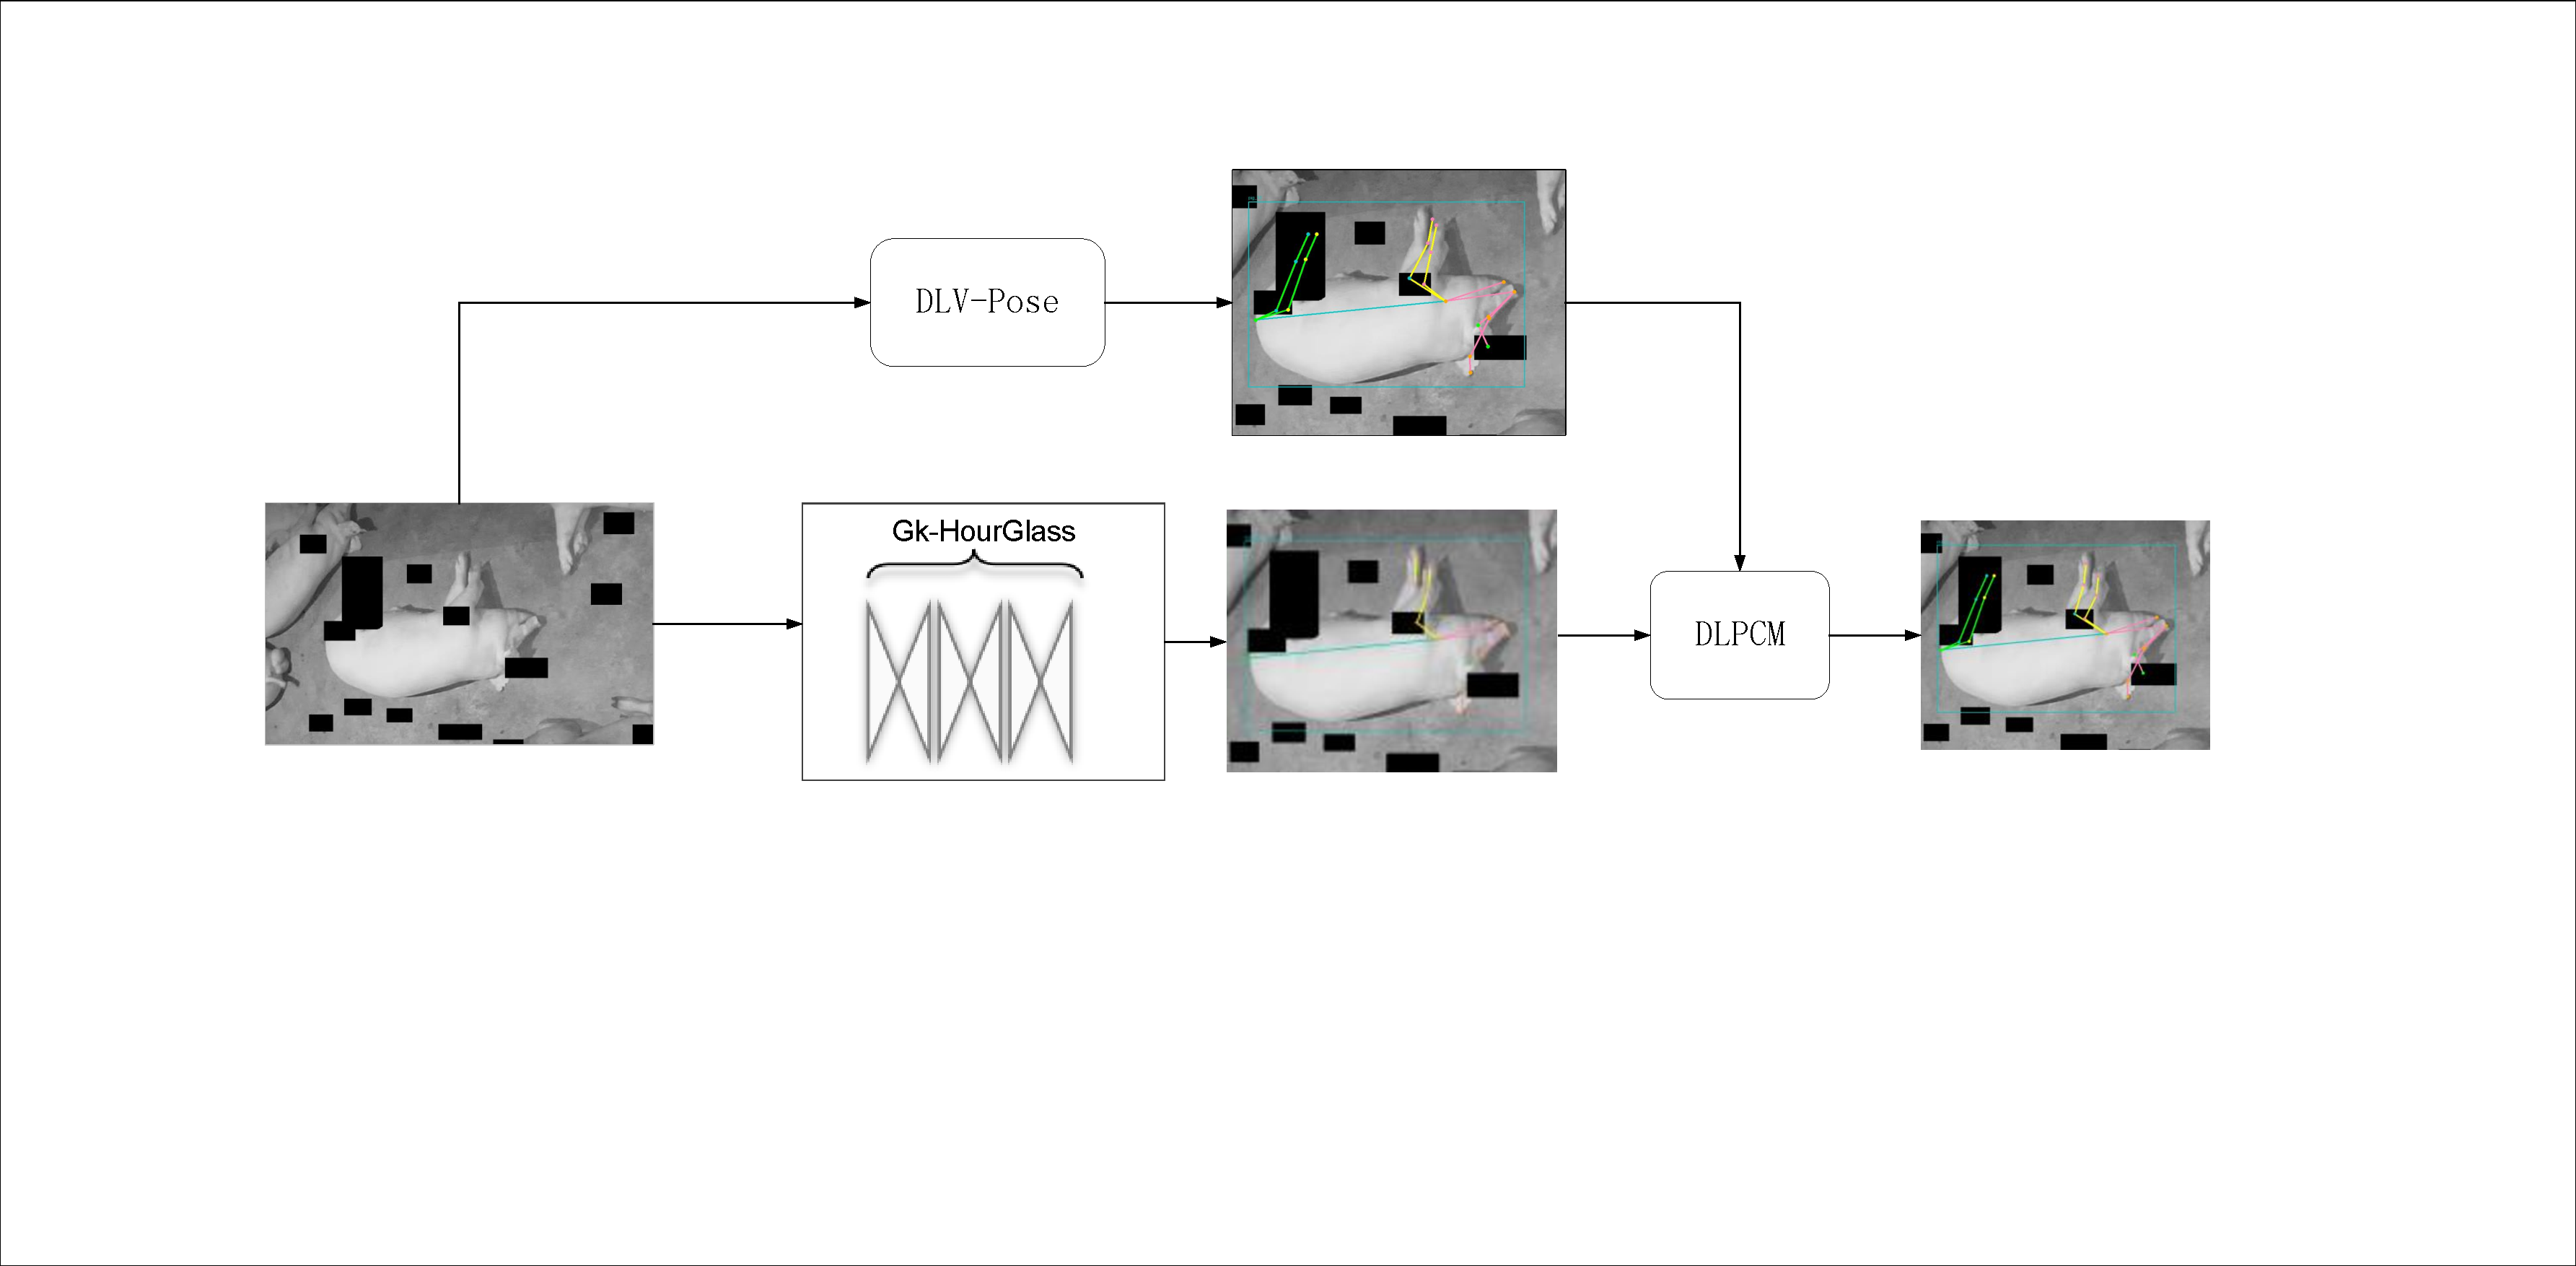
\includegraphics[width=\textwidth,trim=1cm 11cm 1cm 1cm,clip]{fig/fig3.pdf}
\caption{Mask-based occluded keypoint completion and fusion mechanism. DLPCM retains visible keypoints predicted by the SMAL-Pig keypoint head and completes only occluded keypoints using the discrete latent codebook. The visibility mask ($M_v$) controls which keypoints are retained versus completed, ensuring that reliable image-based predictions are preserved while missing keypoints are inferred from structural relationships.}
\label{fig:dlpcm_fusion}
\end{figure}

The masked completion-and-fusion mechanism illustrated in Figure~\ref{fig:dlpcm_fusion} shows how visible keypoints predicted by the SMAL-Pig head are retained, while occluded keypoints are imputed from the discrete latent codebook and merged via the visibility mask.

\subsection{Skeleton Joint-Angle Constraint (SC)}\label{sec:sc}

Although DLPCM restores missing 2D structure, improved 2D completeness does not by itself guarantee plausible 3D pose. Under single-view depth ambiguity, local texture sparsity, and occlusion noise, the regressor may still produce reverse bending, over-rotation, or limb twisting. We therefore introduce a skeleton joint-angle constraint (SC) during pose regression.

In this work, SC specifically regularizes local joint rotations; it does not include any bone-length or global scale constraints. Inter-individual skeletal proportions are captured by SMAL-Pig shape parameters, so SC focuses on suppressing abnormal local rotations rather than restricting natural morphological variation.

Because limb joints have larger degrees of freedom than the trunk and are more sensitive to occlusion-induced errors, the constraint is applied to major limb joints, including shoulder, elbow, hip, and stifle (knee). Let $R_j$ denote the local rotation matrix of joint $j$ in SMAL-Pig. We convert it to an axis--angle vector $\omega_j$ and measure the rotation magnitude using the L2 norm:

\begin{equation}
a_j = \|\omega_j\|_2
\end{equation}

where $a_j$ denotes the magnitude of local rotation for joint $j$. Given the maximum rotation threshold $a_j^{\max}$ allowed for that joint, the rotation overshoot is defined as:

\begin{equation}
\Delta a_j = \max(0, a_j - a_j^{\max})
\end{equation}

The skeleton joint-angle constraint loss is then expressed as:

\begin{equation}
L_{\text{SC}} = L_{\text{angle}} = \frac{1}{|S|} \sum_{j \in S} [\max(0, a_j - a_j^{\max})]^2
\end{equation}

where $S$ is the set of limb joints subject to the constraint. The rotation thresholds $a_j^{\max}$ are empirically set from plausible poses observed in training data and validated against biomechanics literature on pig and similar quadruped joint mobility.

Note that SC acts as a soft training loss on axis--angle pose parameters in SMAL-Pig rather than a hard post-processing constraint at inference. It is not intended to be a full biomechanical range-of-motion model; instead, thresholds are validated against quadruped biomechanics literature to ensure they reflect physiological limits rather than training artifacts.

\subsubsection{Biomechanical Validation of Joint-Angle Thresholds}\label{sec:biomech_validation}

To validate whether the rotation thresholds $a_j^{\max}$ reflect true biomechanical constraints, we establish the correspondence between SMAL-Pig axis--angle representation and actual pig joint angles. For a joint with axis--angle norm $a_j$ (in radians), the equivalent rotation angle is $\theta_j = a_j \times (180/\pi)$ degrees. The rotation thresholds are empirically set from plausible poses observed in training data and validated against biomechanics literature on pig and similar quadruped joint mobility.

According to biomechanics literature on pig and similar quadruped gait analysis \cite{ref29,ref30,ref31}, typical joint angle ranges during normal locomotion are as follows:

\begin{itemize}
  \item \textbf{Stifle (knee):} flexion range 0$^\circ$--120$^\circ$; typical gait range 20$^\circ$--80$^\circ$.
  \item \textbf{Elbow:} flexion range 0$^\circ$--110$^\circ$; typical gait range 15$^\circ$--70$^\circ$.
  \item \textbf{Hip:} flexion range 0$^\circ$--150$^\circ$; typical gait range 30$^\circ$--90$^\circ$.
  \item \textbf{Shoulder:} flexion range 0$^\circ$--140$^\circ$; typical gait range 20$^\circ$--100$^\circ$.
\end{itemize}

The rotation thresholds used in this work are shown in Table~\ref{tab:biomech_thresholds}. These thresholds are conservative relative to maximum physiological range and cover typical activity ranges in normal pig movement and posture. The design of thresholds aims to suppress pathological or clearly implausible poses, such as reverse knee bending and excessive local twisting, while allowing natural postural variation within reasonable ranges.

\begin{table}[H]
\caption{Rotation thresholds and biomechanical validation.}
\label{tab:biomech_thresholds}
\centering
\small
\begin{tabular}{lcccc}
\toprule
\textbf{Joint} & \textbf{Threshold $a_j^{\max}$ (rad)} & \textbf{Equiv. angle ($^\circ$)} & \textbf{Lit. range ($^\circ$)} & \textbf{Validation} \\
\midrule
Stifle (knee) & 0.90 & 51.6 & 0--120 & $\checkmark$ In range \\
Elbow & 0.80 & 45.8 & 0--110 & $\checkmark$ In range \\
Hip & 1.20 & 68.7 & 0--150 & $\checkmark$ In range \\
Shoulder & 1.00 & 57.3 & 0--140 & $\checkmark$ In range \\
\bottomrule
\end{tabular}
\end{table}

\subsection{Training Strategy and Loss Functions}\label{sec:training}

Training proceeds in two stages. Stage 1 trains the 2D modules, including the SMAL-Pig keypoint head and the DLPCM for occluded keypoint completion. Concretely, GK-HourGlass predicts keypoints and visibilities, while the DLPCM branch learns to infer occluded keypoints using the completion loss in Eq. (13).

Stage 2 integrates the trained 2D modules into the BARC-style weakly supervised 3D reconstruction framework. Similar to BARC using a fixed Stacked-HourGlass module for 2D heatmaps, silhouettes, and intermediate features during 3D training, our 2D modules are not updated by 3D losses. DLPCM retains visible keypoints from the SMAL-Pig head via masked fusion and replaces only the occluded ones with completed estimates, acting as a fixed pre-processing and fusion step during 3D training.

Following BARC, the 3D network is optimized using 2D supervision comprising keypoint reprojection consistency, silhouette consistency, and regularization on shape/pose and camera parameters. With SC introduced, the overall 3D loss is:

\begin{equation}
L_{\text{3D}} = L_{\text{rec}} + \lambda_s L_{\text{SC}}
\end{equation}

Here, $L_{\text{rec}}$ denotes the base BARC-style reconstruction objective (keypoint reprojection, silhouette consistency, and regularizers), and $\lambda_s$ is the weight of SC. In our formulation, $L_{\text{SC}}$ contains only the joint-angle constraint, without bone-length or scale terms.

Therefore, our method should be viewed as an occlusion-oriented extension to a BARC-style weakly supervised parametric reconstruction pipeline rather than an entirely new paradigm: DLPCM enhances the completeness of 2D structural inputs, while SC regularizes local rotations to curb reverse bending and twisting. Together they provide a more stable balance between projection consistency and pose plausibility under occlusion.

\section{Results and Analysis}\label{sec:results}

To validate the effectiveness of our method, we organize experiments in a progressive manner. First, 2D occluded keypoint prediction experiments evaluate whether DLPCM provides more reliable keypoint estimates under occlusion. Second, we conduct ablation studies on 3D reconstruction to analyze whether completed occluded keypoints improve SMAL-Pig reconstruction. Finally, we assess the contribution of SC from the perspectives of pose parameter plausibility and qualitative visualization. Since real farm images lack dense 3D ground truth, we interpret 3D reconstruction results primarily through 2D projection consistency, silhouette consistency, and pose plausibility.

\subsection{2D Occluded Keypoint Prediction Experiments}\label{sec:2d_keypoint}

\subsubsection{Experimental Setup and Metrics}\label{sec:2d_setup}

To assess the effectiveness of the discrete latent completion strategy in DLPCM, we evaluate on a pig image test set with natural and synthetic occlusions. This experiment focuses on the 2D stage: we compare conventional heatmap-based keypoint prediction with the DLPCM-assisted strategy across multiple backbones (HourGlass, Stacked-HourGlass, HR-Former, and GK-HourGlass). Occlusion types include self-occlusion, inter-animal occlusion, and rail occlusion. For fairness, all settings (data split, input resolution, augmentations, backbone configs) are identical except for the keypoint prediction strategy.

Instances are cropped by annotated bounding boxes and resized to 256 $\times$ 256. The DLPCM completion branch is trained with AdamW; both training and validation batch sizes are 32 for 210 epochs. The codebook, decoder, and the classifier head in the second stage are randomly initialized. To accelerate training, the second-stage backbone is initialized from a model pre-trained for 210 epochs on the pig pose dataset with the heatmap method. Early layers are frozen and the last layer is fine-tuned. The initial learning rate is $1 \times 10^{-3}$ with LinearLR warm-up for 500 iterations (ratio 0.001), followed by cosine decay with a minimum LR ratio of $1 \times 10^{-5}$ (final LR $\geq 1 \times 10^{-8}$). Augmentations include cutout (4 $\times$ 4 tiles covering 20\% area) and random hue scaling in [0.9, 1.1]. GK-HourGlass training follows the staged supervision used in Stacked-HourGlass. All experiments run on a workstation with an NVIDIA V100 GPU.

We report AP, AP50, AP75, AP(S), AP(M), and AP(L) on all annotated keypoints of the test set. AP is the average precision over OKS thresholds from 0.50 to 0.95 with a step of 0.05. AP50 and AP75 are AP at OKS = 0.50 and 0.75, respectively, with AP75 being more sensitive to localization errors. AP(S), AP(M), and AP(L) correspond to small, medium, and large targets.

\subsubsection{Keypoint Results Across Backbones}\label{sec:2d_results}

DLPCM-assisted strategy and conventional heatmap strategy results on the occluded-pig test set are shown in Table~\ref{tab:2d_keypoint}. Across all four backbones, DLPCM-assisted prediction consistently outperforms conventional heatmaps. For HourGlass, DLPCM raises AP from 33.2 to 37.9 and AP75 from 23.3 to 31.8, indicating improved high-precision localization. With the stronger GK-HourGlass backbone, DLPCM still improves AP from 37.9 to 42.2, demonstrating broad adaptability.

By target scale, DLPCM generally improves AP(S), AP(M), and AP(L). For HourGlass, AP(S) increases from 20.9 to 25.4 and AP(L) from 40.9 to 47.8; with GK-HourGlass, AP(L) reaches 50.8. These results suggest that the discrete latent completion not only refines local keypoint estimates but also reinforces global structural consistency under occlusion.

In summary, heatmap-only methods rely on local image evidence and thus struggle under missing or weak signals in occluded regions. DLPCM, by modeling inter-keypoint structure, infers invisible or weakly visible keypoints. To avoid potential bias on visible keypoints from a finite codebook, the subsequent 3D stage applies DLPCM only to occluded keypoints via masked fusion, while preserving visible keypoints from the SMAL-Pig head.

\begin{table}[H]
\caption{2D keypoint prediction on the occluded-pig test set: DLPCM-assisted vs heatmap baselines.}
\label{tab:2d_keypoint}
\centering
\small
\setlength{\tabcolsep}{4.5pt}
\begin{tabular}{llcccccc}
\toprule
\textbf{Method} & \textbf{Backbone} & \textbf{AP} & \textbf{AP50} & \textbf{AP75} & \textbf{AP(S)} & \textbf{AP(M)} & \textbf{AP(L)} \\
\midrule
Heatmap-based & HourGlass & 33.2 & 78.3 & 23.3 & 20.9 & 41.1 & 40.9 \\
DLPCM-assisted & HourGlass & 37.9 & 81.6 & 31.8 & 25.4 & 42.3 & 47.8 \\
Heatmap-based & Stacked-HourGlass & 37.8 & 82.9 & 31.6 & 23.2 & 42.1 & 46.5 \\
DLPCM-assisted & Stacked-HourGlass & 41.3 & 85.0 & 34.8 & 27.9 & 44.1 & 50.2 \\
Heatmap-based & HR-Former & 37.4 & 82.5 & 30.9 & 24.8 & 43.4 & 44.2 \\
DLPCM-assisted & HR-Former & 40.8 & 84.2 & 33.9 & 28.3 & 44.7 & 48.1 \\
Heatmap-based & GK-HourGlass & 37.9 & 81.3 & 34.1 & 25.6 & 48.2 & 48.5 \\
DLPCM-assisted & GK-HourGlass & 42.2 & 84.0 & 38.2 & 27.0 & 49.3 & 50.8 \\
\bottomrule
\end{tabular}
\end{table}

\subsection{3D Reconstruction under Occlusion}\label{sec:3d_recon}

\subsubsection{Reconstruction Method and Metrics}\label{sec:3d_method}

In the 3D stage, we adopt SMAL-Pig as the parametric mesh model and regress shape, local pose, and global pose parameters to synthesize pig meshes. Supervision is obtained by projecting the mesh to the image plane and comparing projected keypoints and silhouettes with annotations. DLPCM completes 2D keypoints in occluded regions to strengthen constraints for pose regression, while SC regularizes local joint angles to improve pose plausibility.

All 3D experiments use the same data splits, preprocessing, backbone, optimizer, schedule, and base loss weights under a BARC-style weak supervision protocol. Inputs are resized to 256 $\times$ 256. We train with RMSprop for 220 epochs with an initial learning rate of $5 \times 10^{-4}$, batch size 12, zero momentum, and no weight decay. The learning rate decays by 0.1 at epochs 150, 175, and 200. Thus, performance differences primarily reflect the effects of DLPCM and SC.

Because dense 3D ground truth aligned to single RGB images is unavailable in real farm settings, we do not use absolute 3D geometric errors as primary metrics. Instead, we evaluate from three complementary perspectives: PCK (keypoint reprojection accuracy, using PCK@0.1), IoU (silhouette consistency), and JRVR (rate of joint-rotation violations in the SMAL-Pig local pose parameter space for major limb joints). JRVR is defined as:

\begin{equation}
\text{JRVR} = \left[\frac{1}{M \times |S|}\right] \sum_{n=1}^{M} \sum_{j \in S} I(a_{n,j} > a_j^{\max}) \times 100\%
\end{equation}

Here, $M$ is the number of test samples, $S$ is the set of evaluated limb joints, $a_{n,j}$ is the axis--angle norm for joint $j$ in sample $n$, $a_j^{\max}$ is its threshold, and $I(\cdot)$ is an indicator function. We focus on stifle (knee), elbow, hip, and shoulder joints due to their importance in locomotion. Since JRVR is related to the SC objective, we treat it as an auxiliary plausibility metric and interpret it together with PCK/IoU and qualitative visualizations.

\subsubsection{Ablation Study}\label{sec:ablation}

To validate the contributions of DLPCM and SC to single-view 3D pig reconstruction, we design four ablation settings. The baseline corresponds to a BARC-style SMAL-Pig reconstruction network without DLPCM or SC. The other settings are: (i) DLPCM only, (ii) SC only, and (iii) both DLPCM and SC. Results are shown in Table~\ref{tab:ablation}.

All ablation models use identical data splits, initialization strategies, training schedules, and evaluation protocols. The only varying factors are whether DLPCM is used for occluded keypoint completion and whether the skeleton joint-angle constraint is included in the 3D reconstruction loss.

Compared with the unconstrained baseline, adding DLPCM improves PCK from 61.85\% to 66.73\% and IoU from 64.04\% to 67.90\%. The +DLPCM setting does not replace all keypoints with codebook reconstructions; instead, it retains visible keypoints predicted by the SMAL-Pig keypoint branch and completes only occluded keypoints. This design is based on the fact that when codebook capacity is limited, naive codebook-based reconstruction may bias even visible keypoints. By preserving reliable image-based visible keypoints and completing only missing ones, DLPCM provides more stable 2D structure observations for SMAL-Pig pose regression, improving keypoint projection accuracy and silhouette consistency. Meanwhile, JRVR decreases from 69.74\% to 24.34\%, indicating that 2D structure completion also alleviates occlusion-induced abnormal poses to some extent. This decrease shows that many abnormal rotations in the baseline are induced by incomplete or unreliable 2D observations, not solely by pose priors.

Adding SC alone achieves PCK = 64.79\% and IoU = 66.32\%, both above the baseline. This shows that the skeleton joint-angle constraint does not severely damage image observation consistency. More importantly, JRVR decreases from 69.74\% to 12.50\%, a relative reduction of approximately 82.1\%. This demonstrates that SC effectively suppresses over-rotation, reverse bending, and local twisting by constraining joint-angle magnitudes in the SMAL-Pig pose space, thereby improving 3D pose plausibility.

Combining DLPCM and SC yields the lowest JRVR of 9.38\%, a relative reduction of approximately 86.5\% compared to the unconstrained baseline. However, this model achieves PCK = 64.91\% and IoU = 66.05\%, lower than the DLPCM-only model, indicating that SC introduces a trade-off between projection accuracy and pose plausibility. Combining DLPCM and SC achieves the lowest JRVR of 9.38\% with competitive PCK (64.91\%) and IoU (66.05\%), reflecting a principled trade-off between projection accuracy and pose plausibility. DLPCM mainly enhances structural completeness and silhouette matching, whereas SC primarily reduces abnormal local rotations, jointly improving pose stability under complex occlusions.

\begin{table}[H]
\caption{Ablation results: effects of DLPCM and SC on single-view pig 3D reconstruction.}
\label{tab:ablation}
\centering
\small
\begin{tabular}{llcccc}
\toprule
\textbf{Method} & \textbf{2D keypoint source} & \textbf{SC} & \textbf{PCK / \%} & \textbf{IoU / \%} & \textbf{JRVR / \%} \\
\midrule
Baseline & SMAL-Pig head (all) & $\times$ & 61.85 & 64.04 & 69.74 \\
+DLPCM & SMAL-Pig vis.\ + DLPCM occ. & $\times$ & 66.73 & 67.90 & 24.34 \\
+SC & SMAL-Pig head (all) & $\checkmark$ & 64.79 & 66.32 & 12.50 \\
+DLPCM+SC & SMAL-Pig vis.\ + DLPCM occ. & $\checkmark$ & 64.91 & 66.05 & 9.38 \\
\bottomrule
\end{tabular}
\end{table}

\subsection{Qualitative Visualization of Reconstruction Results}\label{sec:qualitative}

To verify the adaptability of the proposed method in complex farming environments, three typical occlusion scenarios were selected for visualization: pig self-occlusion, occlusion by other pigs, and pen-rail (fence) occlusion. As shown in Figure~\ref{fig:occlusion}, the proposed method recovers relatively continuous 3D pig poses under all three scenarios, with fewer backward-bending or local-twisting artifacts in the leg-joint regions.

\begin{figure}[H]
\centering
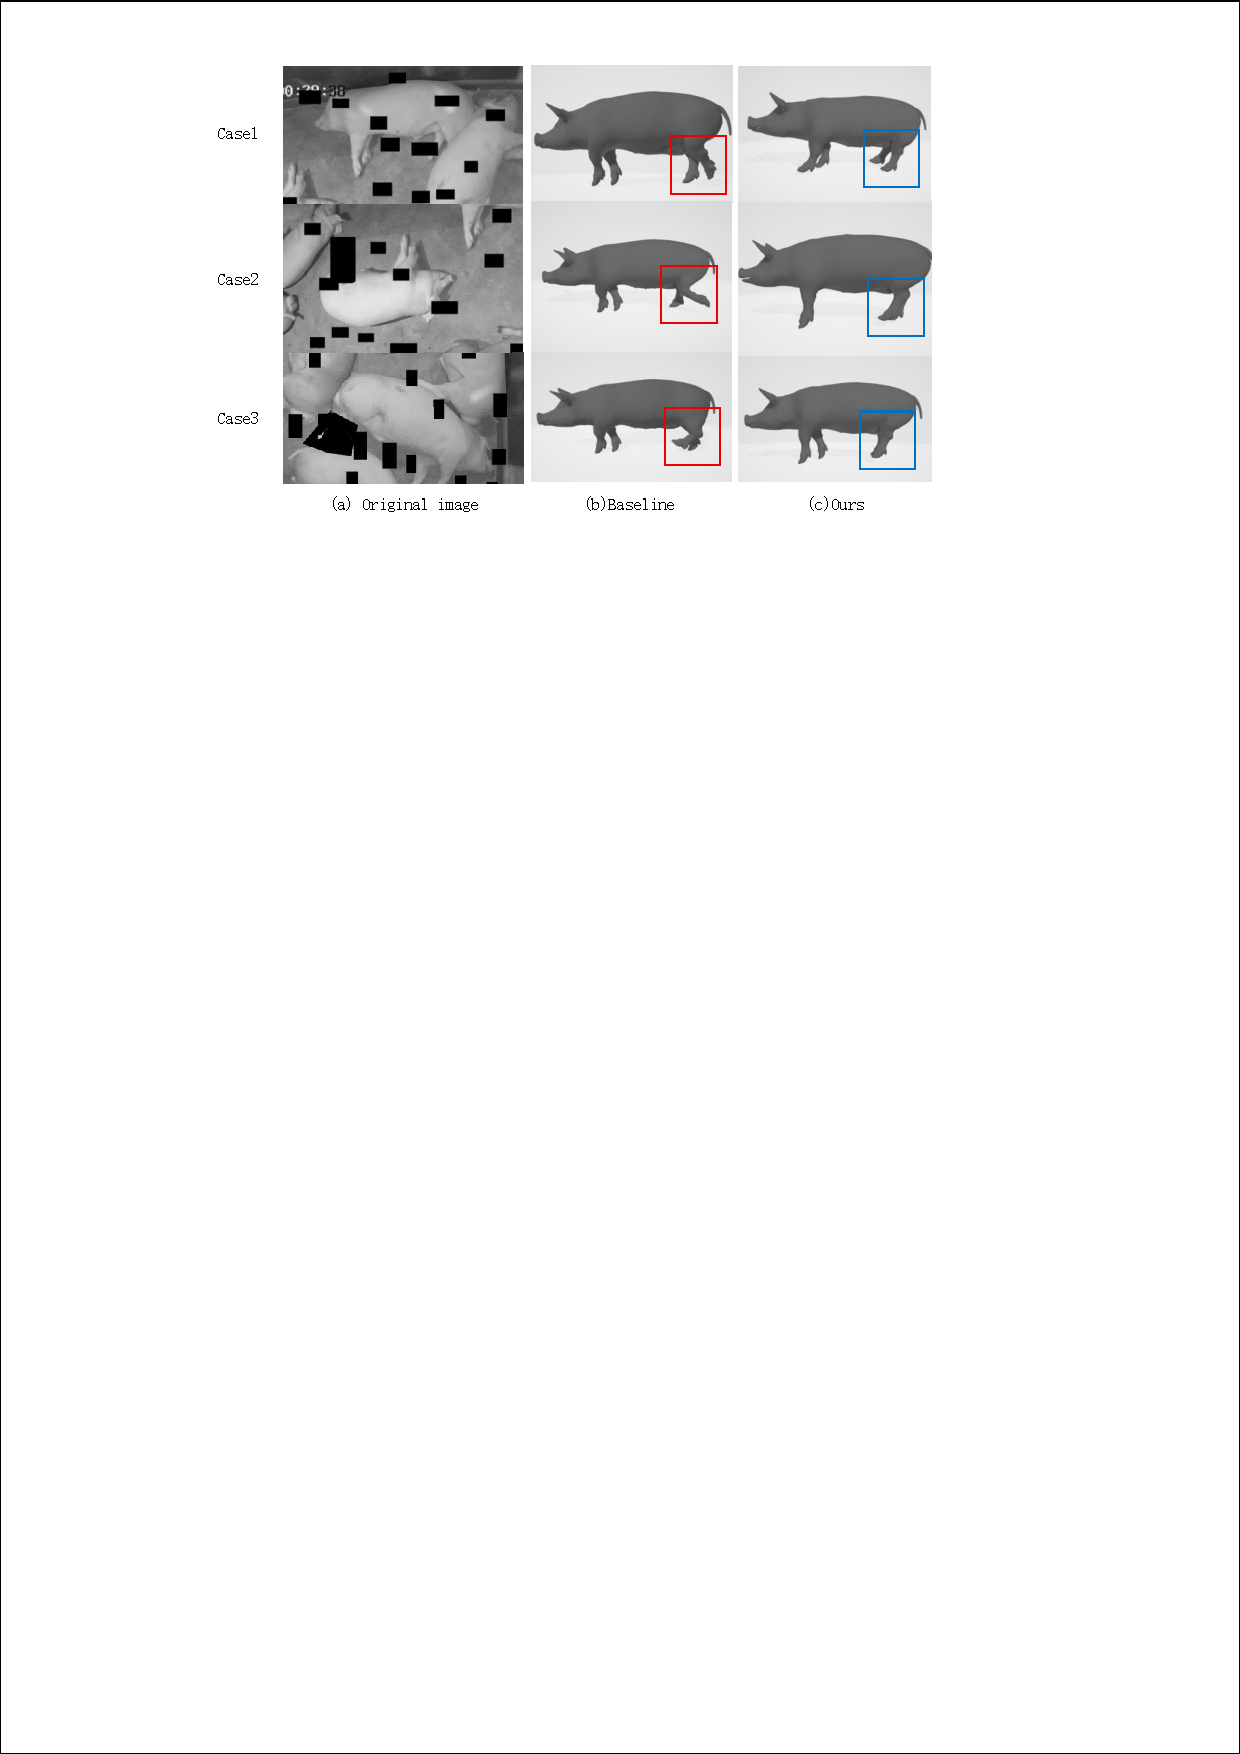
\includegraphics[width=\textwidth]{fig/DLPCM.pdf}
\caption{3D pose reconstruction of pigs under occlusion. (\textbf{a}) Pig self-occlusion; (\textbf{b}) occlusion by other pigs; (\textbf{c}) pen-rail (fence) occlusion. The proposed method recovers continuous 3D poses with fewer backward-bending or local-twisting artifacts than the baseline.}
\label{fig:occlusion}
\end{figure}

To further examine performance under severe local occlusion, artificial occlusion was added to test images, mainly covering the leg-joint regions so that some leg keypoints became invisible. The same image was reconstructed with the original SMAL-Pig network and with the SMAL-Pig network integrated with DLPCM, as shown in Figure~\ref{fig:dlpcm_effect}. Without DLPCM, the baseline tends to produce joint-position deviations and local pose distortions due to insufficient 2D observations; after incorporating DLPCM, the recovered leg joints become more continuous because occluded keypoints are inferred from the structural relationships among visible keypoints.

\begin{figure}[H]
\centering
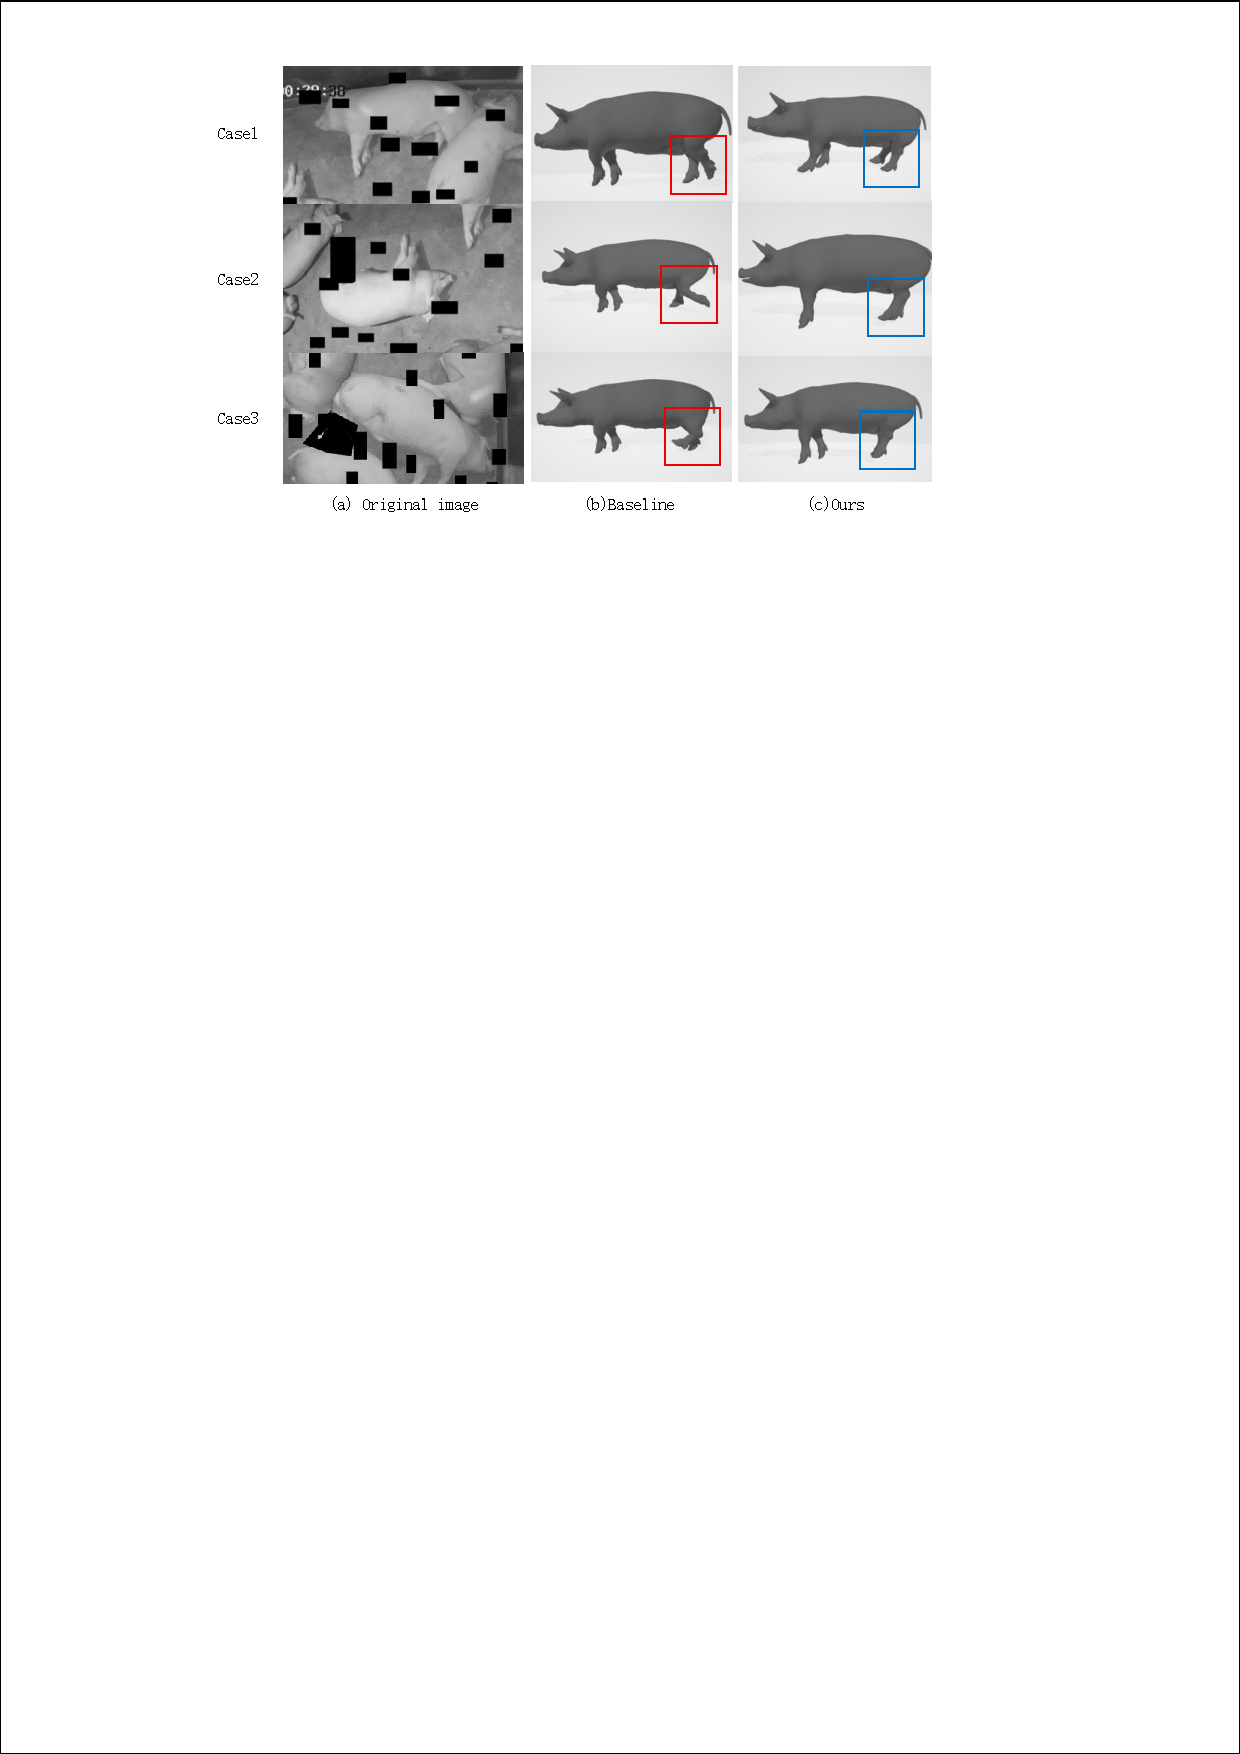
\includegraphics[width=\textwidth,trim=3cm 21cm 3cm 1cm,clip]{fig/DLPCM.pdf}
\caption{Effect of DLPCM on 3D reconstruction. (\textbf{a}) Original image; (\textbf{b}) baseline SMAL-Pig without DLPCM, showing joint-position deviations in occluded leg regions; (\textbf{c}) result after incorporating DLPCM, with more continuous leg joints. Visible keypoints are retained from the SMAL-Pig keypoint branch, while occluded keypoints are completed by DLPCM.}
\label{fig:dlpcm_effect}
\end{figure}

Figure~\ref{fig:sc_effect} shows the reconstruction after adding the skeleton joint-angle constraint. Compared with the unconstrained result, SC restricts abnormal rotations of major leg joints such as the hip and knee and brings distorted regions closer to plausible poses, indicating that the main role of SC is to reduce abnormal local rotation patterns in the pose-parameter space rather than merely improving 2D projection metrics.

\begin{figure}[H]
\centering
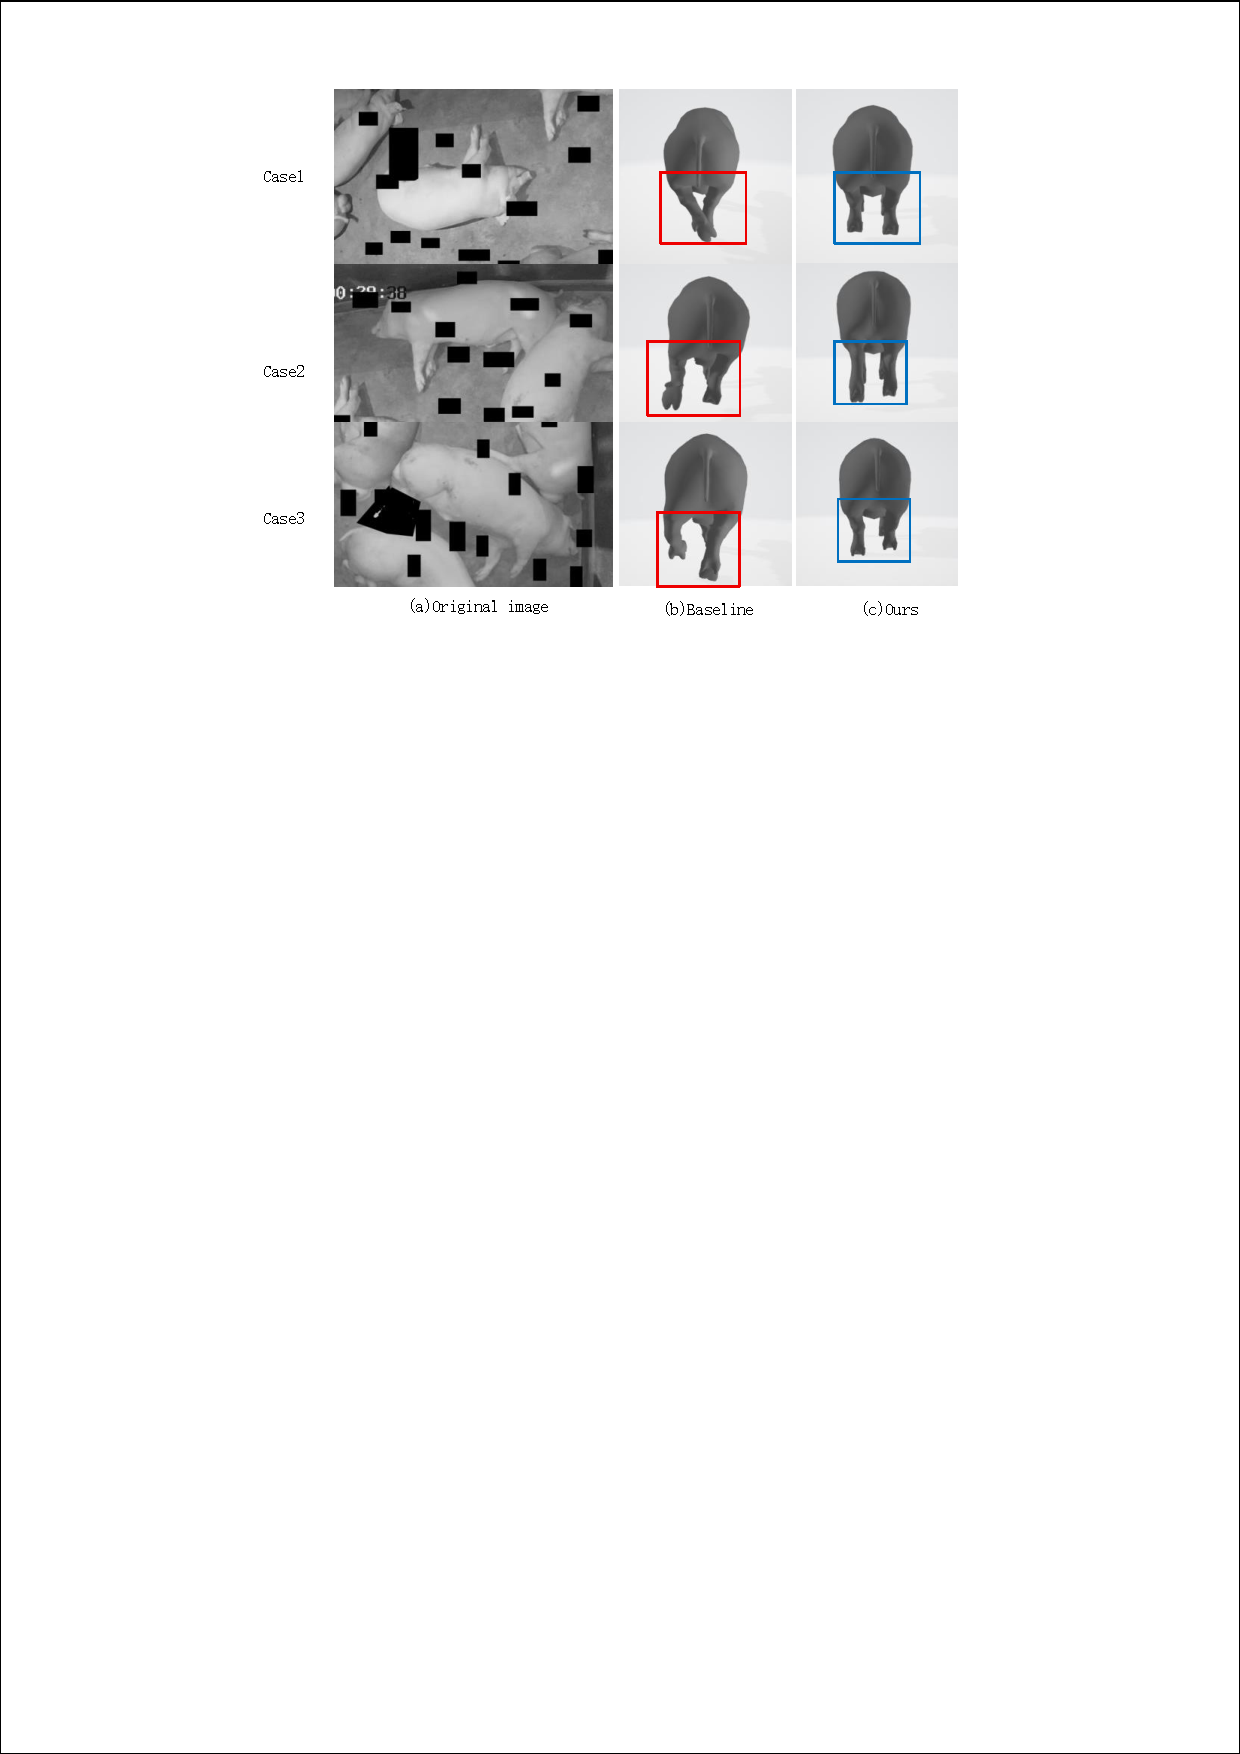
\includegraphics[width=\textwidth,trim=4cm 18cm 1cm 1cm,clip]{fig/sc.pdf}
\caption{3D pig pose reconstruction with the skeleton joint-angle constraint (SC). Compared with unconstrained results, SC restricts abnormal rotations of major leg joints (hip, knee) and reduces distorted regions to plausible poses.}
\label{fig:sc_effect}
\end{figure}

Finally, Figure~\ref{fig:multiview} provides a multi-view visualization of the reconstruction with SC. The method recovers relatively plausible 3D pig poses even when image information is incomplete. Combined with the quantitative experiments, DLPCM mainly improves structural observations in occluded regions, while SC mainly reduces abnormal joint rotations; together they improve pose stability for single-view 3D pig reconstruction in complex farming environments.

\begin{figure}[H]
\centering
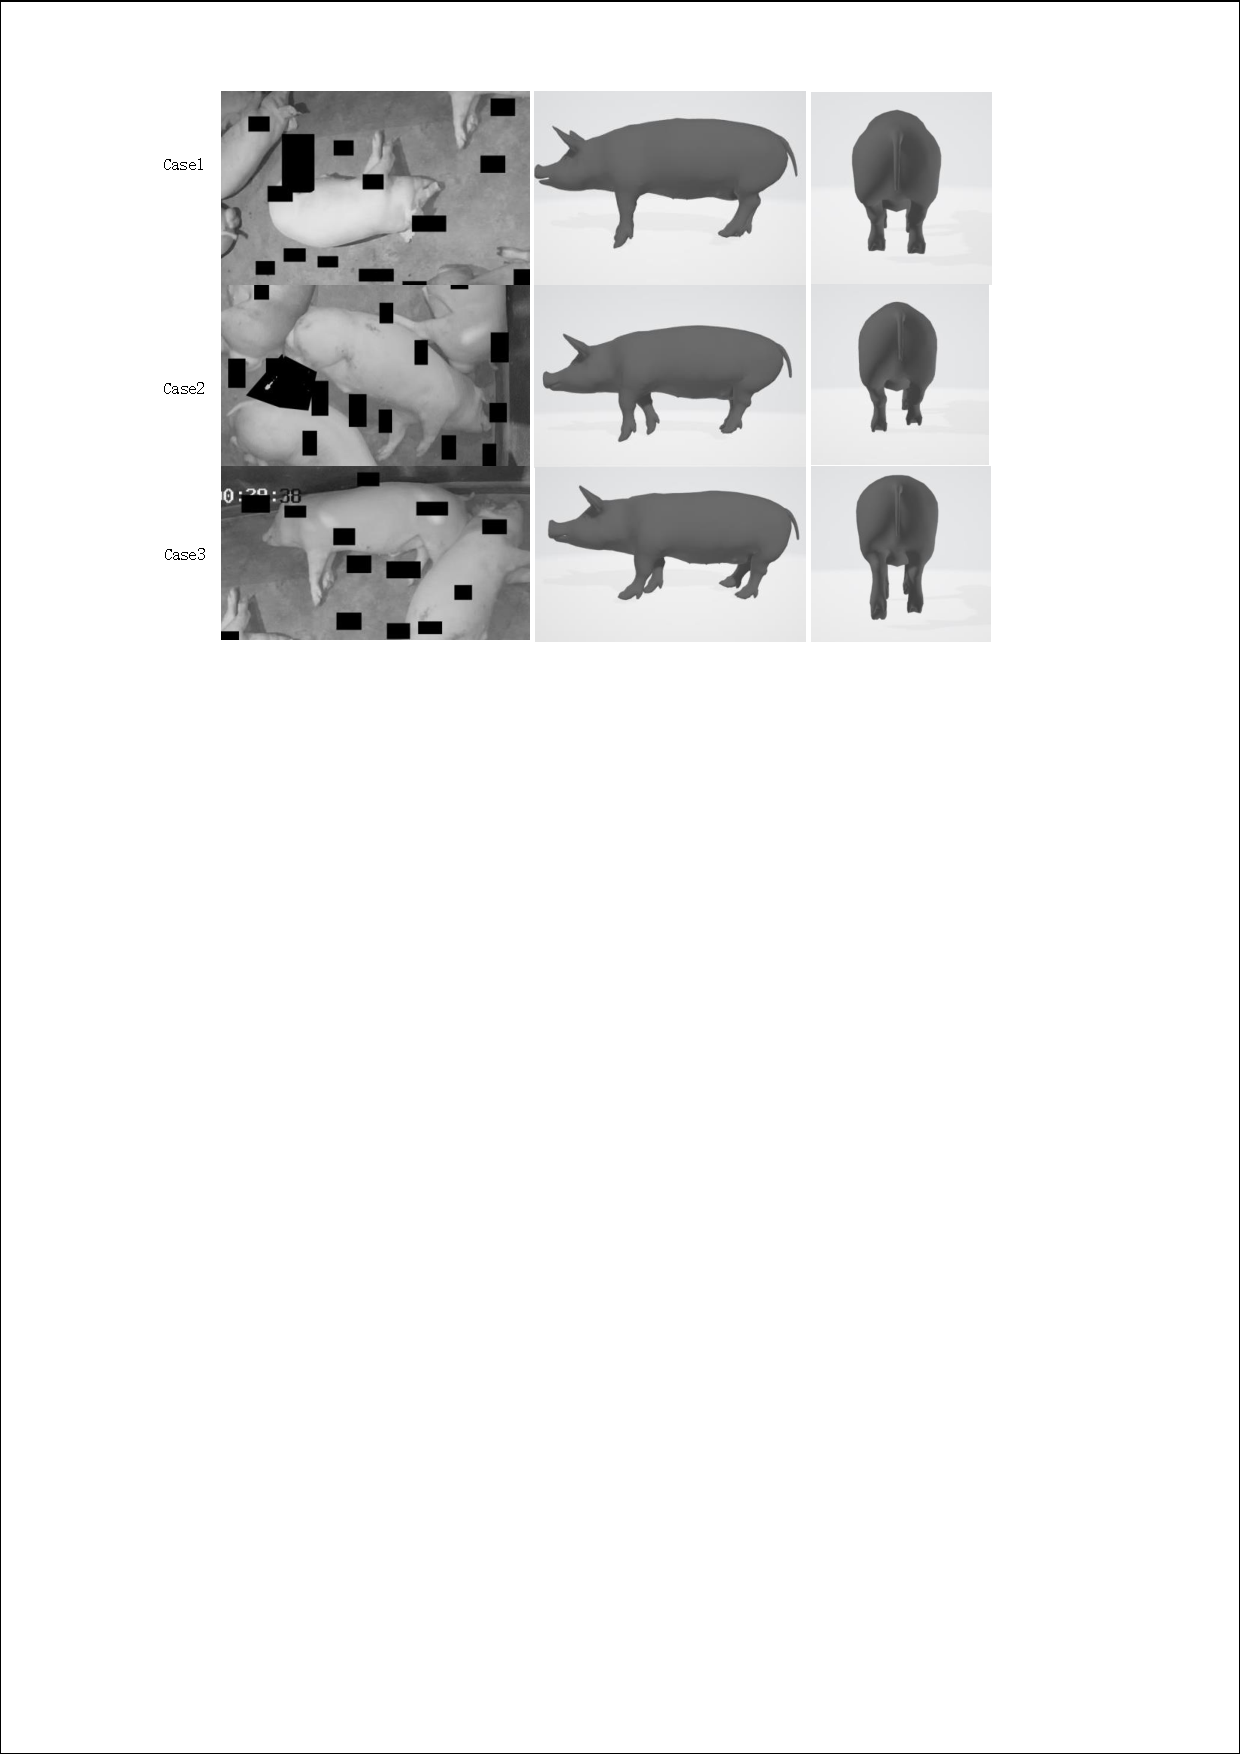
\includegraphics[width=\textwidth,trim=1cm 18cm 1cm 1cm,clip]{fig/DLCPM_SC.pdf}
\caption{Multi-view visualization of 3D pig pose reconstruction with the skeleton joint-angle constraint. (\textbf{a}) Original image; (\textbf{b}) side view showing plausible limb configurations; (\textbf{c}) rear view demonstrating pose stability under occlusion.}
\label{fig:multiview}
\end{figure}

\section{Discussion}\label{sec:discussion}

Our occlusion-robust single-view 3D reconstruction framework addresses a critical challenge in precision livestock farming: robust pose estimation under real-world occlusion. By integrating DLPCM and SC, we achieve a better balance between 2D projection consistency and 3D pose plausibility.

\textbf{Key Findings:} DLPCM improves 2D structural completeness by inferring occluded keypoints from visible structure, while SC regularizes local rotations to suppress anatomically implausible configurations. Their combination yields the most stable reconstructions under complex occlusions.

\textbf{Limitations and Future Work:} Open challenges remain under severe occlusion, heavy overlap, or very sparse visibility. Given the lack of dense 3D ground truth, our evaluation emphasizes 2D projection and plausibility measures. Future directions include exploiting temporal cues, multi-frame consistency, denser 3D supervision where feasible, and instance separation in crowded barns.

\section{Conclusions}\label{sec:conclusions}

We address missing 2D structure and implausible 3D poses caused by occlusion in real pig-house imagery with an occlusion-robust single-view 3D reconstruction method. Building on the SMAL-Pig parametric model, our approach integrates a Discrete Latent Pose Completion Module (DLPCM) to complete occluded keypoints and a skeleton joint-angle constraint (SC) to regularize local rotations.

Experiments demonstrate improved projection consistency and pose plausibility under occlusion. With DLPCM only, PCK rises from 61.85\% to 66.73\% and IoU from 64.04\% to 67.90\%, while JRVR drops from 69.74\% to 24.34\%. This indicates that DLPCM leverages structural relations among visible keypoints to infer occluded ones, providing more complete 2D constraints for 3D regression while preserving visible keypoints from the image-based head.

With SC only, PCK = 64.79\% and IoU = 66.32\%, both above baseline, and JRVR falls to 12.50\%, showing that SC effectively suppresses over-rotation, reverse bending, and local twisting by constraining joint-angle magnitudes in the SMAL-Pig pose space.

Combining DLPCM and SC yields the lowest JRVR of 9.38\% with competitive PCK (64.91\%) and IoU (66.05\%), reflecting a principled trade-off between projection accuracy and pose plausibility. DLPCM mainly enhances structural completeness and silhouette matching, whereas SC primarily reduces abnormal local rotations, jointly improving pose stability under complex occlusions.

\authorcontributions{Conceptualization, Ge Wang, Tao Zhu and Fuchuan Ni; methodology, Ge Wang; software, Ge Wang; validation, Ge Wang and Tao Zhu; formal analysis, Ge Wang; investigation, Ge Wang; resources, Fuchuan Ni; data curation, Ge Wang; writing---original draft preparation, Ge Wang; writing---review and editing, Tao Zhu and Fuchuan Ni; visualization, Ge Wang; supervision, Fuchuan Ni. All authors have read and agreed to the published version of the manuscript.}

\funding{This research received no external funding.}

\institutionalreview{Not applicable.}

\informedconsent{Not applicable.}

\dataavailability{Data and code are available from the corresponding author upon reasonable request.}

\acknowledgments{We thank the farm staff for assistance in data collection and annotation.}

\conflictsofinterest{The authors declare no conflict of interest.}

\reftitle{References}

\begin{thebibliography}{99}

\bibitem{ref1} Li, B.M.; Wang, Y.; Zheng, W.C.; et al. Research progress on intelligent equipment and information technology for livestock and poultry farming. \textit{Journal of South China Agricultural University} \textbf{2021}, \textit{42}(6), 1--15.

\bibitem{ref2} Yang, L.; Wang, H.; Chen, R.P.; et al. Research progress of intelligent pig farming factories. \textit{Journal of South China Agricultural University} \textbf{2023}, \textit{44}(2), 1--12.

\bibitem{ref3} Guo, Y.Y.; Du, S.Z.; Qiao, Y.L.; et al. Research and application progress of deep learning in intelligent livestock farming. \textit{Smart Agriculture} \textbf{2023}, \textit{5}(1), 1--18.

\bibitem{ref4} Zhang, J.L.; Zhuang, Y.R.; Zhou, K.; et al. Design and experiment of a fattening pig grouping system based on machine vision. \textit{Transactions of the Chinese Society of Agricultural Engineering} \textbf{2020}, \textit{36}(17), 196--203.

\bibitem{ref5} Yao, Y.P.; Xu, C.; Chen, H.J.; et al. Pig body-size estimation based on keypoint detection and multi-object tracking. \textit{Journal of South China Agricultural University} \textbf{2024}, \textit{45}(5), 722--729.

\bibitem{ref6} Hu, Z.X.; Xiang, L.; Yang, B.; et al. Multi-view voxel-based 3D skeleton reconstruction for pig lameness detection. \textit{Transactions of the Chinese Society of Agricultural Engineering} \textbf{2024}, \textit{45}(5), 703--715.

\bibitem{ref7} Liu, L.S.; Liu, L.; Zhou, J.; et al. Research progress on intelligent perception technologies for precision sow farming. \textit{Journal of South China Agricultural University} \textbf{2024}, \textit{45}(5), 690--702.

\bibitem{ref8} Zhao, C.J.; Li, D.L.; Liu, G.; et al. Research on the development status and strategic objectives of smart agriculture. \textit{Strategic Study of CAE} \textbf{2018}, \textit{20}(2), 1--8.

\bibitem{ref9} Qin, C.Y.; Chen, M.; Zhang, M.; et al. Research progress on the application of computer vision technology in modern agriculture. \textit{Journal of Chinese Agricultural Mechanization} \textbf{2023}, \textit{44}(12), 160--170.

\bibitem{ref10} Wang, C.; Zhang, M.; Li, H.; et al. Research progress on automatic measurement technology of livestock body size. \textit{Transactions of the Chinese Society of Agricultural Engineering} \textbf{2022}, \textit{38}(13), 255--268.

\bibitem{ref11} Liang, J.; Yuan, Z.; Luo, X.; et al. A study on the 3D reconstruction strategy of a sheep body based on a Kinect v2 depth camera array. \textit{Animals} \textbf{2024}, \textit{14}(17), 2457.

\bibitem{ref12} Qi, C.R.; Yi, L.; Su, H.; Guibas, L.J. PointNet++: Deep hierarchical feature learning on point sets in a metric space. In \textit{Proceedings of the 31st International Conference on Neural Information Processing Systems}; 2017; pp. 5105--5114.

\bibitem{ref13} Hao, H.; Yang, J.; Yin, L.; et al. An improved PointNet++ point cloud segmentation model applied to automatic measurement method of pig body size. \textit{Computers and Electronics in Agriculture} \textbf{2023}, \textit{205}, 107560.

\bibitem{ref14} Jiang, Y.; Li, Z.; Cao, J.; et al. Body parts segmentation and phenotypic trait extraction of pig using an improved point cloud segmentation network with multi-LiDAR. \textit{Computers and Electronics in Agriculture} \textbf{2025}, \textit{237}, 110624.

\bibitem{ref15} Nath, T.; Mathis, A.; Chen, A.C.; et al. Using DeepLabCut for 3D markerless pose estimation across species and behaviors. \textit{Nature Protocols} \textbf{2019}, \textit{14}, 2152--2176.

\bibitem{ref16} Karashchuk, P.; Rupp, K.L.; Dickinson, E.S.; et al. Anipose: A toolkit for robust markerless 3D pose estimation. \textit{Cell Reports} \textbf{2021}, \textit{36}(13), 109730.

\bibitem{ref17} Waldmann, U.; Chan, A.H.H.; Naik, H.; et al. 3D-MuPPET: 3D multi-pigeon pose estimation and tracking. \textit{International Journal of Computer Vision} \textbf{2024}, \textit{132}, 4235--4252.

\bibitem{ref18} An, L.; Ren, J.; Yu, T.; et al. Three-dimensional surface motion capture of multiple freely moving pigs using MAMMAL. \textit{Nature Communications} \textbf{2023}, \textit{14}, 7727.

\bibitem{ref19} Loper, M.; Mahmood, N.; Romero, J.; et al. SMPL: A skinned multi-person linear model. \textit{ACM Transactions on Graphics} \textbf{2015}, \textit{34}(6), 248.

\bibitem{ref20} Zuffi, S.; Kanazawa, A.; Jacobs, D.W.; et al. 3D Menagerie: Modeling the 3D shape and pose of animals. In \textit{Proceedings of the IEEE Conference on Computer Vision and Pattern Recognition}; 2017; pp. 6365--6373.

\bibitem{ref21} Zuffi, S.; Kanazawa, A.; Black, M.J. Lions and tigers and bears: Capturing non-rigid, 3D, articulated shape from images. In \textit{Proceedings of the IEEE Conference on Computer Vision and Pattern Recognition}; 2018.

\bibitem{ref22} Zuffi, S.; Kanazawa, A.; Berger-Wolf, T.; et al. Three-D Safari: Learning to estimate zebra pose, shape, and texture from images in the wild. In \textit{Proceedings of the IEEE/CVF International Conference on Computer Vision}; 2019.

\bibitem{ref23} Biggs, B.; Boyne, O.; Charles, J.; et al. Who left the dogs out? 3D animal reconstruction with expectation maximization in the loop. In \textit{European Conference on Computer Vision}; 2020.

\bibitem{ref24} Li, C.; Lee, G.H. Coarse-to-fine animal pose and shape estimation. In \textit{Advances in Neural Information Processing Systems}; 2021; Vol. 34, pp. 11757--11768.

\bibitem{ref25} Ruegg, N.; Zuffi, S.; Schindler, K.; et al. BARC: Learning to regress 3D dog shape from images by exploiting breed information. In \textit{Proceedings of the IEEE/CVF Conference on Computer Vision and Pattern Recognition}; 2022; pp. 3876--3884.

\bibitem{ref26} Ruegg, N.; Tripathi, S.; Schindler, K.; et al. BITE: Beyond priors for improved three-D dog pose estimation. In \textit{Proceedings of the IEEE/CVF Conference on Computer Vision and Pattern Recognition}; 2023; pp. 8867--8876.

\bibitem{ref27} Wu, S.; Li, R.; Jakab, T.; et al. MagicPony: Learning articulated 3D animals in the wild. In \textit{Proceedings of the IEEE/CVF Conference on Computer Vision and Pattern Recognition}; 2023.

\bibitem{ref28} Rong, Z.Y.; He, Z.D.; Zhu, T.; et al. Occluded pig pose estimation based on neural discrete representation learning. \textit{Transactions of the Chinese Society of Agricultural Engineering} \textbf{in press}, 1--12. doi:10.11975/j.issn.1002-6819.202503129.

\bibitem{ref29} Fadeev, I.; Streijger, F.; Shortt, K.; et al. Gait analysis in swine, sheep, and goats after neurologic injury: Validation of a novel, non-invasive kinematic analysis system. \textit{Journal of Neuroscience Methods} \textbf{2020}, \textit{338}, 108703.

\bibitem{ref30} Thorson, J.F.; Lowe, J.B.; Schroeder, A.L.; et al. Treadmill-based gait kinematics in the Yucatan mini pig: Locomotor parameters and kinematic patterns during bipedal and quadrupedal gait. \textit{Journal of Biomechanics} \textbf{2023}, \textit{155}, 111627.

\bibitem{ref31} Hildebrand, M. The Quadrupedal Gaits of Vertebrates: The Timing of Limb Cycles During Locomotion. \textit{Biological Reviews} \textbf{1989}, \textit{64}(2), 143--195.

\bibitem{ref32} Mathis, A.; Mamidanna, P.; Cury, K.M.; et al. DeepLabCut: markerless pose estimation of user-defined body parts with deep learning. \textit{Nature Neuroscience} \textbf{2018}, \textit{21}(9), 1281--1289.

\bibitem{ref33} Graving, J.M.; Chae, D.; Naik, H.; et al. DeepPoseKit: a software toolkit for fast and robust animal pose estimation using deep learning. \textit{eLife} \textbf{2019}, \textit{8}, e47994.

\bibitem{ref34} Pereira, T.D.; Shaevitz, J.W.; Murthy, M. Quantifying behavior to understand the brain. \textit{Nature Neuroscience} \textbf{2020}, \textit{23}(12), 1537--1549.

\bibitem{ref35} Kingma, D.P.; Welling, M. Auto-encoding variational Bayes. \textit{arXiv preprint arXiv:1312.6114} \textbf{2013}.

\bibitem{ref36} Oord, A.V.D.; Vinyals, O.; Kavukcuoglu, K. Neural discrete representation learning. In \textit{Advances in Neural Information Processing Systems}; \textbf{2017}; Vol. 30, pp. 6306--6315.

\end{thebibliography}

\end{document}
